\documentclass[final]{fhnwreport}       %[mode] = draft or final
                                        %{class} = fhnwreport, article, 
                                        %          report, book, beamer, standalone
%%---Main Packages-----------------------------------------------------------------------
\usepackage[english, ngerman]{babel}	%Mul­tilin­gual sup­port for LaTeX
\usepackage[T1]{fontenc}				%Stan­dard pack­age for se­lect­ing font en­cod­ings
\usepackage[utf8]{inputenc}				%Ac­cept dif­fer­ent in­put en­cod­ings
\usepackage{lmodern}                    %The newer Font-Set
\usepackage{textcomp}					%LaTeX sup­port for the Text Com­pan­ion fonts
\usepackage{caption}					%Customising captions in floating environments

\usepackage{graphicx} 					%En­hanced sup­port for graph­ics
\usepackage{float}						%Im­proved in­ter­face for float­ing ob­jects
\usepackage{ifdraft}                    %Let you check if the doc is in draft mode

%%---Useful Packages---------------------------------------------------------------------
\usepackage{color}						%Colour control for LaTeX documents
\usepackage[pdftex,dvipsnames]{xcolor}  %Driver-in­de­pen­dent color ex­ten­sions for LaTeX
\usepackage{csquotes}                   %Simpler quoting with \enquote{}
\usepackage{siunitx} 					%A com­pre­hen­sive (SI) units pack­age
\usepackage{listings}					%Type­set source code list­ings us­ing LaTeX
\usepackage[bottom]{footmisc}			%A range of foot­note op­tions
\usepackage{footnote}					%Im­prove on LaTeX's foot­note han­dling
\usepackage{verbatim}					%Reim­ple­men­ta­tion of and ex­ten­sions to LaTeX ver­ba­tim
\usepackage[textsize=footnotesize]{todonotes} %Mark­ing things to do in a LaTeX doc­u­ment
\usepackage{titling}					%Control over the typesetting of the \maketitle command

\usepackage{float}
\usepackage{wrapfig}

%%---Tikz Packages-----------------------------------------------------------------------
\usepackage{standalone}
\usepackage{tikz}
\usepackage{circuitikz}
\usetikzlibrary{arrows}
\usetikzlibrary{calc}
\usetikzlibrary{intersections}

%%---Math Packages-----------------------------------------------------------------------
\usepackage{amsmath}					%AMS math­e­mat­i­cal fa­cil­i­ties for LaTeX
\usepackage{amssymb}					%Type­set­ting symbols (AMS style)
%\usepackage{amstext}
%\usepackage{amsfonts}
%\usepackage{breqn}
\usepackage{array}						%Ex­tend­ing the ar­ray and tab­u­lar en­vi­ron­ments
\usepackage{amsthm}					%Type­set­ting the­o­rems (AMS style)

%%---Table Packages----------------------------------------------------------------------
\usepackage{tabularx}					%Tab­u­lars with ad­justable-width columns
%\usepackage{longtable}
\usepackage{multirow}					%Create tab­u­lar cells span­ning mul­ti­ple rows
\usepackage{multicol}					%In­ter­mix sin­gle and mul­ti­ple columns

%%---PDF / Figure Packages---------------------------------------------------------------
\usepackage{pdfpages}					%In­clude PDF doc­u­ments in LaTeX
\usepackage{pdflscape}					%Make land­scape pages dis­play as land­scape
\usepackage{subfig}					    %Fig­ures di­vided into sub­fig­ures

%%---Other Packages----------------------------------------------------------------------
%\usepackage{xargs}                     %De­fine com­mands with many op­tional ar­gu­ments


%%---Bibliography------------------------------------------------------------------------
\usepackage[style=ieee,urldate=comp,backend=biber]{biblatex}
\addbibresource{literature/bibliography.bib}

%%---Main Settings-----------------------------------------------------------------------
\graphicspath{{./graphics/}}			%Defines the graphicspath
\geometry{twoside=false}				    %twoside=false disables the "bookstyle"
\setlength{\marginparwidth}{2cm}
\overfullrule=5em						%Creates a black rule if text goes over the margins => debugging




%%---User Definitions--------------------------------------------------------------------
%%Tabel-Definitions: (requires \usepackage{tabularx})
\newcolumntype{L}[1]{>{\raggedright\arraybackslash}p{#1}}    %column-width and alignment
\newcolumntype{C}[1]{>{\centering\arraybackslash}p{#1}}
\newcolumntype{R}[1]{>{\raggedleft\arraybackslash}p{#1}}

%%---Optional Package Settings-----------------------------------------------------------
%Listings-Settings: (requires \usepackage{listings}) => Example with Matlab Code
\lstset{language=Matlab,%
    basicstyle=\footnotesize\ttfamily,
    breaklines=false,%
    morekeywords={switch, case, otherwise},
    keywordstyle=\color{Blue},%
    tabsize=2,
    %morekeywords=[2]{1}, keywordstyle=[2]{\color{black}},
    identifierstyle=\color{Black},%
    stringstyle=\color{Purple},
    commentstyle=\color{Green},%
    showstringspaces=false,%without this there will be a symbol in the places where there is a space
    numbers=left,%
    numberstyle={\tiny \color{black}},% size of the numbers
    numbersep=9pt, % this defines how far the numbers are from the text
    %emph=[1]{word1, word2,...},emphstyle=[1]\color{red}
}							

%Hurenkinder und Schusterjungen verhindern (kein Scherz, Google es)
\clubpenalty10000
\widowpenalty10000
\displaywidowpenalty=10000	



%Titel mit Mathematik immer fett drucken
\usepackage{sectsty}
\allsectionsfont{\boldmath}




			                %loads all packages, definitions and settings											
\title{Fachbericht}  		        %Project Title
\author{Team 1}      				    %Document Type => Technical Report, ...
\date{\today}          				   %Place and Date

\begin{document}

%%---TITLEPAGE---------------------------------------------------------------------------------
\thispagestyle{empty}
%	\ohead{\includegraphics[scale=0.5]{Bilder/Logo_FHNW.jpg}}
	\begin{figure}
		 \vspace*{-\topskip}\vspace*{-\headsep}
		
\includegraphics[scale=1]{graphics/fhnw_ht_logo_de.pdf}
	\end{figure}
	\begin{center}
		\vspace*{2cm}
		{\huge{\textbf{digitales Theremin}}}\\
		\vspace*{0.2cm}
		{\huge{\textbf{\thetitle}}}\\
		\vspace*{0.5cm}
		
		{\scshape\Large Projekt 6\\} \Large{\today}
		\vfill
		\begin{normalsize}
			{\begin{tabbing}
					\textbf{Auftraggeber:} \hspace{5cm}\= Prof. Dr. Hanspeter Schmid\\
					
					\\[0.8cm]
					\textbf{Betreuung:} 
					\>Prof. Dr. Hanspeter Schmid\\
					\>Prof. Karl Schenk\\
					
					\\[0.8cm]
					\textbf{Experte:} 
					\>Dr. Jürg M. Stettbacher\\

					\\[0.8cm]
					\textbf{Team:} \>Andreas Frei \\ \>Dennis Aeschbacher \\ 

					\\[0.8cm]
					\textbf{Studiengang:} \>Elektro- und Informationstechnik
					\\[0.8cm]	\textbf{Semester:} \>Frühlingssemester 2020
			\end{tabbing}}
		\end{normalsize}
		\vfill
	\end{center}
\clearpage
			
%%---ABSTRACT----------------------------------------------------------------------------
\selectlanguage{english}				%ngerman or english
\thispagestyle{empty}
\begin{abstract}
% Description aim/objective
\noindent In this Project a Theremin was built that mainly operates on digital hardware unlike the original device that solely used analog electronics. The device is supposed to be used in presentations for trade fairs by the Institute for Sensors and Electronics ISE. As such the device should be built in a appealing housing. Moreover the device should have other additional functionality such as soundeffects or the ability to record sound.
% Method
The digital hardware was implemented in VHDL on the developer board DE1-SoC from terasIC with a Cyclone V FPGA from Intel. The sole analog component implemented was the oscillator that controls the pitch. 
% Results
The pitch of the device can be changed well, but the sound itself has a flaw at the moment, because there is an audible crackle. This is due to a communication problem with the codec that was used for the audio output. This problem will not be corrected during this project, because the communication will be implemented differently in the finished product.
% Conclusion
The work in this project served as a platform for the continuation in project 6. The next steps would be to implement the volume control and redesign the pcb for two antennas and oscillators.


\end{abstract}	



%%---TABLE OF CONTENTS-------------------------------------------------------------------
\pagenumbering{Roman}		
\selectlanguage{ngerman}				%ngerman or english
\tableofcontents
\clearpage

%%---TEXT--------------------------------------------------------------------------------
\pagenumbering{arabic}
\clearpage
\section{Einleitung}\label{sec:Einleitung}
Das Theremin kennen heutzutage nur wenige Leute, obwohl es das erste elektronische Instrument war. Es wurde 1920 von dem Russen Lev Sergejewitsch Termen, welcher sich später zu Leon Theremin umbenennen liess, erfunden \cite{Theremin_h}. Personen die regelmässig Filme schauen, haben die Musik welche mit einem Theremin gemacht wird bestimmt schon einmal gehört. Ein Beispiel dafür ist Ghostbusters, wo das Theremin oft im Hintergrund zu hören ist. Zudem ist das Theremin in einigen Science-Fiction-Filmen und Horrorfilmen zu hören \cite{Goast_m}. Das Theremin wird ohne es zu berühren gespielt, indem man mit den Händen die Distanz zu zwei Antennen ändert. Dies führt zu Veränderung der Tonhöhe und Lautstärke.

Im Projekt 5 und 6 soll nun ein solches Instrument entwickelt werden. Mit dem Unterschied, dass das sonst analoge Instrument digital aufgebaut werden soll. Dabei soll es auf einem Field Programmable Gate Array (FPGA) implementiert werden. Später soll das Theremin als Messeobjekt für das Institut für Sensorik und Elektronik ISE verwendet werden. Im Rahmen des Projekt 5 wurde die Tonhöhenantenne des Theremin realisiert. Dazu wurde die Antenne zusammen mit dem Antennenoszillator analog beibehalten. Die restlichen Komponenten wurden in VHDL realisiert. Das Resultat wurde auf dem DE1-SoC Board von terasIC mit einem Cyclone V FPGA von Intel getestet.

Der folgende Fachbericht beginnt mit dem Kapitel \ref{sec:Technische Grundlagen} Technische Grundlagen.In der ersten Hälfte des Kapitel wird erklärt wie ein analoges Theremin funktioniert und welche Komponenten ein Theremin ausmachen. In der zweiten Hälfte werden digitale Lösungsansätze besprochen. Anschliessend wird im Kapitel \ref{sec:Realisierung} Realisierung beschrieben wie die Komponenten realisiert wurden. Im Kapitel \ref{sec:Validierung} Validierung wird als erstes auf die Inbetriebnahme des Antennenoszillators eingegangen. Als nächstes werden die Simulationen des VHDL Codes erläutert. Im letzten Abschnitt wird auf die Inbetriebnahme des VHDL Codes auf dem DE1-SoC Board Bezug genommen.






\pagebreak

	
\clearpage
\section{Technische Grundlagen}\label{sec:Technische Grundlagen}
Um ein Verständnis für dessen Funktionsweise zu gewinnen, ist in diesem Kapitel als erstes erklärt, wie ein analoges Theremin funktioniert. Anschliessend folgt ein kleiner Abschnitt zur Musiktheorie. Zuletzt werden verschiedene Algorithmen erklärt, welche im digitalen Theremin eingesetzt wurden.
	\subsection{analoges Theremin}\label{subsec:Theremin_analog}
Das klassische Theremin besitzt zwei Antennen. Der Spieler kann über die senkrecht angebrachte Antenne  die  Tonhöhe beeinflussen. Mit der waagrechten Antenne beeinflusst der Spieler die Lautstärke. Eine typische Eigenschaft des Theremin ist, dass der Ton des Theremin in einem weitem Frequenzbereich kontinuierlich veränderbar ist. Das Theremin kann daher alle Frequenzen in einem Bereich spielen, im Gegensatz zu den meisten anderen Instrumenten.

Der Spieler spielt das Theremin durch verstimmen der Oszillatoren über die Antennen.
Die Hand des Spielers verändert über die jeweilige Antenne die Schwingfrequenz des Tonhöhen und Lautstärkeoszillators. Dabei wird der kapazitive Anteil des LC-Schwingkreises beeinflusst, was eine Änderung der Schwingfrequenz zur Folge hat. 
Die Frequenz dieser Oszillatoren ist jedoch weit über dem hörbaren Bereich (zwischen \SI{100}{kHz} bis \SI{1}{MHz}). Mit Hilfe eines Mischers und einem Referenzoszillator wird die Frequenzdifferenz des Tonhöhenoszillators hörbar gemacht und danach verstärkt\cite{Franzis}. Der Lautstärkepegel ergibt sich durch die Verwendung eines Bandpassfilters und nachfolgenden Hüllkurvendetektor. Die Abbildung \ref{img:Blockschaltbild_analog} gibt einen Überblick über die Schaltungskomponenten eines Theremins. Die einzelnen Schaltungsteile sind im folgenden Teil genauer erklärt.

\begin{figure}[h]
	\centering
	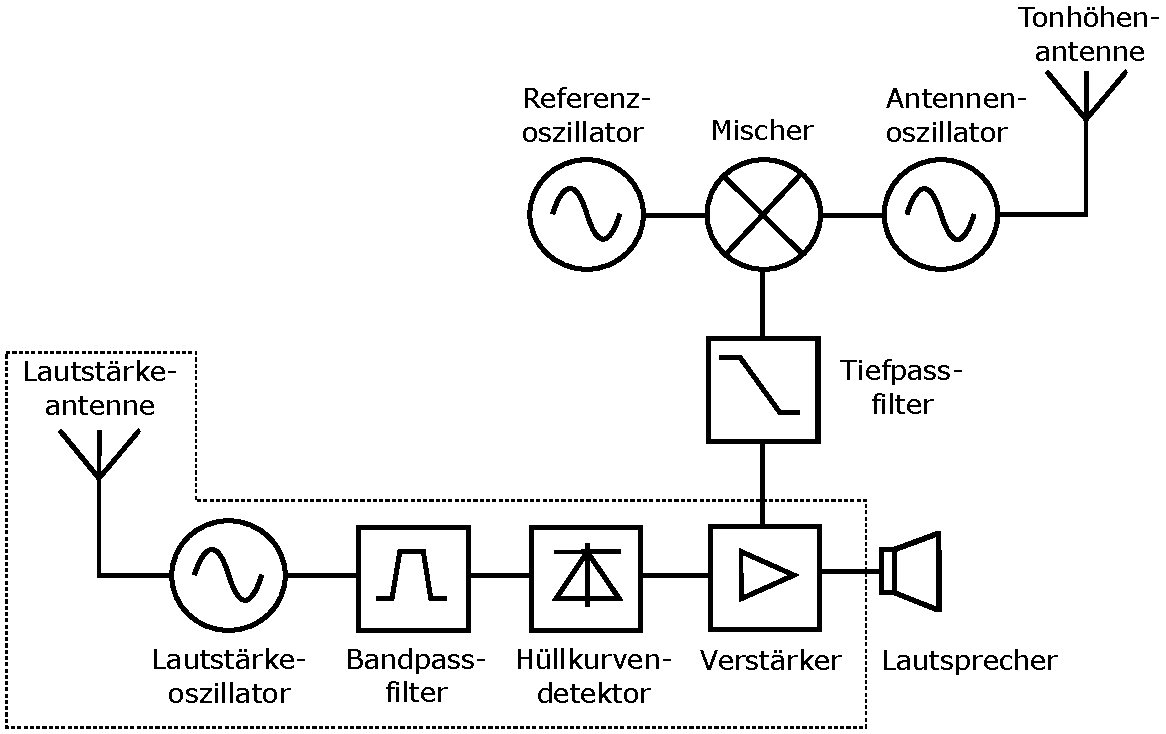
\includegraphics[width=0.8\textwidth]{Blockschaltbild_analog.pdf}
	\caption{Blockschaltbild eines analogen Theremins}
	\label{img:Blockschaltbild_analog}
\end{figure}

\paragraph{Tonhöhenoszillator und Tonhöhenantenne}\mbox{}\\

Die Tonhöhenantenne ist ein Metallrohr welches mit dem Tonhöhenoszillator verbunden ist.
Der Spieler kann über die Distanz seiner Hand zur Antenne die Frequenz des Tonhöhenoszillator verändern. Die über die Antenne zu erreichende Kapazitätsänderung ist sehr gering. Diese liegt im Picofarad Bereich \cite{physik_theremin}.Die Grundfrequenz des Tonhöhenoszillator muss weit über dem hörbaren Bereich liegen, dass eine genügend grosse Frequenzänderung entsteht.

\paragraph{Lautstärkeoszillator und Lautstärkeantenne}\mbox{}\\ 

Die Lautstärkeantenne ist wie die Tonhöhenantenne ein Metallrohr, welches mit dem Lautstärkeoszillator verbunden ist. Die durch den Spieler beeinflusste Frequenzänderung wandelt ein Hüllkurvendetektor in eine Spannung um. Diese Spannung dient dem Verstärker als Steuergrösse um das Audio Signal zu verstärken. \cite{Franzis}. 

\paragraph{Mischer und Referenzoszillator}\mbox{}\\ 
\\Die erzeugte Frequenz der Tonhöhenantenne ist weit über dem vom Menschen hörbaren Bereich. Der Mischer multiplizeirt die Signale des Referenzoszillators und des Tonhöhenoszillators wie in Formel \ref{equ:mischer}. $A_1\sin(\omega_1)$ ist das Signal des Referenzoszillators und $A_2\sin(\omega_2)$ das Signal des Tonhöhenoszillators.

\begin{equation}
V_{out} = A_{1}A_{2} \sin(\omega_{1}t)   \sin(\omega_{2}t) 
\label{equ:mischer}
\end{equation}

$V_{out}$ kann durch Additionstheoreme umgeformt werden. Dabei erhält man folgenden Ausdruck:

\begin{equation}
V_{out} = A/2[\cos((\omega_{1}-\omega_{2})t)  - \cos((\omega_{1}+\omega_{2})t) ]
\label{equ:mischer_trigo}
\end{equation}

Das Ausgangssignal $V_{out}$ hat zwei Frequenzkomponenten. Zum einen die Differenz der beiden Frequenzen zum anderen die Summe der Frequenzen. Dabei ist bei dem Theremin nur die Differenz der Frequenzen von Interesse \cite{physik_theremin}.

Eine Kalibration des Theremins ist vor jedem Gebrauch nötig. Es könnte beispielsweise sein, dass die Differenz der Frequenz ausserhalb des hörbaren Bereiches ist. Dazu stellt der Spieler beim klassischen Theremin mit Hilfe eines Trimmkondensators am Referenzoszillator die Differenzfrequenz auf \SI{0}{Hz} ein.

\paragraph{Tiefpassfilter}\mbox{}\\ 
\\Das Tiefpassfilter filtert die hochfrequente Komponente aus Formel \ref{equ:mischer_trigo} weg. Übrig bleibt die Differenz der Oszillatorfrequenzen. Dieser ist der interessante Anteil des Mischprozesses, da er im hörbaren Bereich ist.
\begin{equation}
V_{out} = A/2cos((\omega_{1}-\omega_{2})t) 
\label{equ:mischer_gefilt}
\end{equation}

\paragraph{Verstärker und  Lautsprecher}\mbox{}\\ 
\\Der Verstärker verstärkt das Ausgangssignal des Tiefpassfilter abhängig von der Spannung, welche vom Hüllkurvendetektor stammt.

	\subsection{Musiktheorie}\label{subsec:Musiktheorie}

Um besser an einem Musikinstrument arbeiten zu können ist es wichtig ein wenig Musiktheorie zu kennen. Der wichtigste Fakt ist wohl, dass der Schallpegel logarithmisch wahrgenommen wird und in Dezibel (dB) gemessen wird. Auch die Frequenz der Tonhöhe hören wir nicht linear. Ein Ton mit \SI{400}{Hz} nehmen wir nicht als doppelt so hoch wahr als ein Ton mit \SI{200}{Hz}. Dies ist sehr schön ersichtlich in Tabelle \ref{tab:Toene_Frequenzen}. Je höher die Töne werden, desto grösser werden die Frequenzunterschiede. Für einfacheres Rechnen von diesen Unterschieden wird die Masseinheit Cent gebraucht. Dabei ist definiert, dass zwei Töne \SI{100}{Cent} auseinanderliegen und dass zwei Töne mit einer Oktave Unterschied \SI{1200}{Cent} Frequenzunterschied haben. Diese Cent-Werte kann man mithilfe von Formel \ref{equ:Cent} in einen Faktor umrechnen \cite{Cent}.

\begin{equation}
x = \sqrt[\leftroot{-2}\uproot{1}1200]{2}^{n_{cent}}
\label{equ:Cent}
\end{equation} 

Dabei ist \(n_{cent}\) der Unterschied in Cent und \(x\) als Faktor.\\ Ist nun die ``akustische'' Mitte zwischen Zwei Tönen gesucht ist die Berechnung mit Cent nützlich. Diese Mitte liegt nicht linear zwischen den beiden Tönen sondern \SI{50}{Cent} entfernt von beiden Tönen. Werden diese \SI{50}{Cent} in einen Faktor umgerechnet und mit dem tieferen Ton multipliziert erhält man die Mitte.

Um nun zu sagen, wann ein Unterschied in der Frequenz vom Gehör wahrgenommen wird, kommt es ganz auf die Person drauf an. Als Faustformel kann gesagt werden, dass zwei aufeinanderfolgende Töne mit etwa \SI{6}{Cent} unterschied vom Gehör registriert wird.\cite{Cent}

Ein weiteres interessantes Thema ist die Pentatonik. Dabei handelt es sich um ein Tonsystem mit nur 5 Tönen. Als Beispiel kann das Klavier genommen werden. Benützt der Spieler nur die Schwarzen Tasten des Klavier, so würde er in einem pentatonischen Tonsystem spielen. In Abbildung \ref{tab:Toene_Frequenzen} entspricht dies allen Tönen mit einem \# in der Notation. Ein Merkmal der Pentatonik ist, dass es sehr einfach ist eine Melodie zu spielen, die ansprechend klingt, ohne grossen Aufwand.\cite{Pentatonik}



\begin{table}[H]
	\centering
	\caption{Töne aus vier Oktaven und deren Frequenzen \cite{Toene_Frequenzen}}
	\label{tab:Toene_Frequenzen}
	\begin{tabular}{l|l|l|l|l|l}
		\textbf{Ton} & \textbf{Frequenz[Hz]} & \textbf{Ton} & \textbf{Frequenz[Hz]} &\textbf{Ton} & \textbf{Frequenz[Hz]} \\
		\hline\hline
		C3 	& 130.813 	& F4	 & 349.228		& A\#5	 &  932.328	 \\ \hline
		C\#3 & 138.591 	& F\#4	 & 369.994		& B5	 &  987.767	 \\ \hline
		D3 	& 146.832 	& G4	 & 391.995		& C6	 &  1046.5	 \\ \hline
		D\#3 & 155.563 	& G\#4	 & 415.305		& C\#6	 &  1108.73	 \\ \hline
		E3 	& 164.814 	& A4	 & 440		 	& D6	 &  1174.66	 \\ \hline
		F3 	& 174.614 	& A\#4	 & 466.164		& D\#6	 &  1244.51	 \\ \hline
		F\#3 & 184.997 	& B4	 & 493.883		& E6	 &  1318.51	 \\ \hline
		G3 	& 195.998 	& C5	 & 523.251		& F6	 &  1396.91	 \\ \hline
		G\#3 & 207.652 	& C\#5	 & 554.365		& F\#6	 &  1479.98	 \\ \hline
		A3 	& 220 		& D5	 & 587.33		& G6	 &  1567.98	 \\ \hline
		A\#3 & 233.082 	& D\#5	 & 622.254		& G\#6	 &  1661.22	 \\ \hline
		B3 	& 246.942 	& E5	 & 659.255		& A6	 &  1760	 \\ \hline
		C4 	& 261.626 	& F5	 & 698.456		& A\#6	 &  1864.66	 \\ \hline
		C\#4 & 277.183 	& F\#5	 & 739.989		& B6	 &  1975.53	 \\ \hline
		D4 	& 293.665 	& G5	 & 783.991		& C7	 &  2093	 \\ \hline
		D\#4 & 311.127 	& G\#5	 & 830.609		&  		 &  		 \\ \hline
		E4 	& 329.628 	& A5	 & 880		 	&  		 &  		 \\ \hline
	
		
	\end{tabular}
\end{table}
	\subsection{Cordic Algorithmus}\label{subsec:Cordic}

Um in einem FPGA aufwendigere Rechenoperationen wie die Berechnung eines Sinus zu implementieren ist eine zusätzliche Hardware notwendig. Der Cordic Algorithmus kann für diesen Zweck eingesetzt werden. Nebst anderen diversen Rechenoperationen ist der Einsatz als Sinusgenerator möglich, was in späteren Kapiteln genauer besprochen ist. \\
Der Cordic Algorithmus ist ein iterativer Algorithmus welcher praktisch nur Additionen und Verschiebungen von Bits benötigt. 
Er kann in zwei Modi betrieben werden. Zum einen der Vektor Modus, in welchem die Berechnung eines Winkels aus einem gegebenen Vektor möglich ist. Zum anderen der Rotationsmodus, mit welchem aus einem gegebenen Winkel die Elemente des zugehörigen Vektors berechnet werden können. Die folgenden Formeln sind für diese Berechnung notwendig \cite{Cordic}:

\begin{equation}
x_{i+1} = x_i - y_id_i2^{-i}
\label{equ:cordic_1}
\end{equation} 
\begin{equation}
y_{i+1} = y_i + x_id_i2^{-i}
\label{equ:cordic_2}
\end{equation} 
\begin{equation}
z_{i+1} = z_i - d_i\arctan{2^{-i}}
\label{equ:cordic_3}
\end{equation} 

Dabei ist die Berechnung von \(d_i\) im Rotationsmodus wie folgt: 

\begin{equation}
d_i=
\begin{cases}
-1 &z_i < 0 \\
1 &\text{otherwise}
\end{cases}
\label{equ:cordic_4}
\end{equation} 

Formeln \ref{equ:cordic_1} bis \ref{equ:cordic_3} zeigen schön den iterativen Ablauf des Algorithmus auf. Um nun einen Sinuswert zu berechnen sind folgende Initialwerte notwendig:

\begin{equation}
\begin{aligned}
x_0 = 1 \\
y_0 = 0 \\
z_0 = \varphi
\end{aligned}
\label{equ:cordic_3}
\end{equation} 

\(\varphi\) ist der gegebene Winkel, welcher zwischen \(-\pi/2\) und \(\pi/2\) sein muss, damit der Algorithmus konvergiert.

Daraus ergeben sich nach \(n\) Iterationen der Sinus und Kosinus Wert wie folgt:

\begin{equation}
\begin{aligned}
x_n = \frac{\cos{\varphi}}{A} \\
y_n = \frac{\sin{\varphi}}{A}
\end{aligned}
\label{equ:cordic_3}
\end{equation} 

Schlussendlich ist es notwendig die Resultate um den Faktor \(A = 0.60725294\) zu korrigieren um die richtigen Werte zu erhalten.


	\subsection{CIC Filter}\label{subsec:CIC_Filter}

Ein CIC-Filter oder Cascaded-Integrator-Comb-Filter ist ein digitales Filter, welches nebst der Filterung eines Signals zusätzlich deren Abtastfrequenz verändert. Abbildung \ref{img:CIC_Filter} zeigt ein Dezimations-CIC-Filter. Dieses verkleinert die Abtastfrequenz am Ausgang um den Faktor \(R\). Die zweite Form ist ein Interpolation-CIC-Filter. Dieses vergrössert die Abtastfrequenz um den Faktor \(R\).

In Abbildung \ref{img:CIC_Filter} ist zu sehen, dass das Filter in drei Stufen unterteilt ist. Links ist ein Integrator-Filter zu sehen, welches einen anliegenden Wert mit einem verzögerten Wert aufaddiert oder anders gesagt, das Signal integriert. Anschliessend folgt ein Dezimierer, welcher das Signal um den Faktor R unterabtastet. Zuletzt folgt ein Combfilter. Dieses nimmt den aktuellen Wert und subtrahiert den alten Wert. Ein Interpolation-CIC-Filter erhält man durch tauschen von Integrator-Filtern mit Comb-Filtern und umgekehrt. Weiter ist nun in der Mitte eine Überabtastung nötig.\\
Es ist möglich, mehrere Integrator- und Combfilterpaare zusammen zu schalten, um eine grössere Dämpfung höherer Frequenzen zu bewirken. Das CIC-Filter benötigt jedoch, um zu funktionieren, eine gewisse Anzahl Bits in den Speichern der Verzögerungselemente, welche grösser als die Anzahl Eingangsbits ist. Dieser Effekt nennt sich Bit-Growth und die zusätzliche Anzahl Bits lässt sich wie folgt berechnen\cite{cic_a}\cite{cic_h}:

\begin{equation}
B_+ = \big \lceil Nlog_2RM \big \rceil
\label{equ:cic_bitgrowth}
\end{equation}

Dabei entspricht N der Ordnung des Filters oder wie viele Integrator-Comb-Filterpaare das Filter hat. R ist der zuvor genannte Dezimationsfaktor und M ist die Verzögerung der Speicherelemente.

Das CIC-Filter verstärkt das Eingangssignal zudem um einen Faktor \(G\). Dieser lässt sich wie folgt berechnen:

 \begin{equation}
 G = (R\cdot M)^N
 \label{equ:cic_gain}
 \end{equation}
 
Um nun den Faktor zu berechnen, um welchen man den Ausgang eines CIC-Filter multiplizieren muss, um den Zahlenbereich voll auszunutzen, kann folgende Formel eingesetzt werden:

\begin{equation}
G_+ = G/2^{B_+}
\label{equ:cic_gain+}
\end{equation}

Ein Problem, welches die CIC-Filter mit sich bringen, ist, dass sie in bestimmten Situationen Aliasing erzeugen. Dieses entsteht wenn sich Signalkomponenten zu nahe an den Nullstellen des Filters befinden \cite{CIC_Aliasing}. In Abbildung \ref{img:CIC_Filter_plot} sieht man sehr schön, dass sehr auf die Frequenz des Signals im Vergleich zum verwendeten CIC-Filter geachtet werden muss.


\begin{figure}[h]
	\centering
	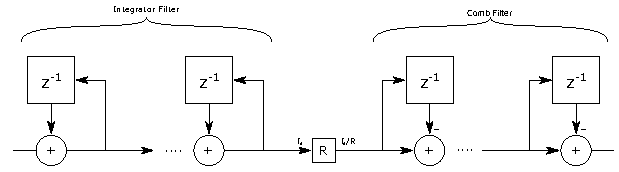
\includegraphics[width=\textwidth]{CIC_Filter.pdf}
	\caption{Aufbau eines CIC-Filters N-ter Ordnung mit Eingang mix\_out und Ausgang filt\_out}
	\label{img:CIC_Filter}
\end{figure}

\begin{figure}[h]
	\centering
	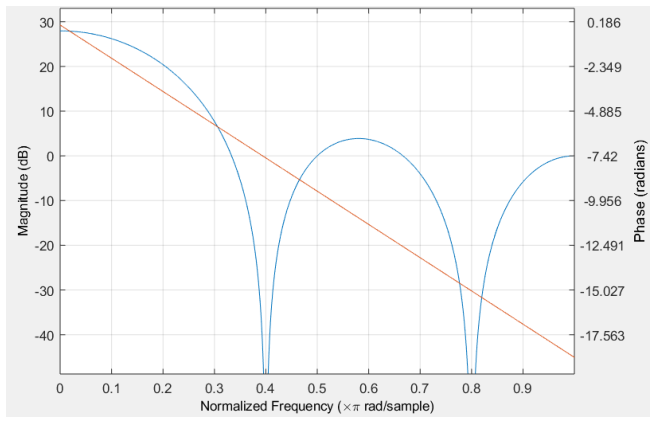
\includegraphics[width=0.9\textwidth]{CIC_Filter_plot.pdf}
	\caption{Amplitudengang und Phasengang eines CIC-Filters (M = 1, R = 5; N = 2)}
	\label{img:CIC_Filter_plot}
\end{figure}

\clearpage

	\subsection{Goldschmidt Algorithmus}\label{subsec:Goldschmidt}

Um in FPGAs dividieren zu können ist es nötig selber eine solche Operation zu implementieren. Dafür gibt es für verschiedene Anforderungen diverse Algorithmen. Einer dieser ist der Goldschmidt Algorithmus. Er ermöglicht es iterativ eine Division zweier Zahlen durchzuführen welche als Resultat auch Nachkommazahlen enthält. Für die Berechnung multipliziert der Algrithmus den Nenner und Zähler wie in Formel \ref{equ:golds_Q} iterativ mit den Faktoren \(F_n\).

\begin{equation}
Q = \frac{Z}{N}\frac{F_1}{F_1}\frac{F_2}{F_2}\frac{F_3}{F_3}\frac{F_{...}}{F_{...}}
\label{equ:golds_Q}
\end{equation}

Offensichtlich verändert dies nicht das Verhältnis des Zählers und Nenners. Für die Berechnung einer Iteration ergeben sich folgende Formeln:

\begin{equation}
F_{i+1} = 2 - N_i
\label{equ:golds_Fi+1}
\end{equation}
\begin{equation}
Z_{i+1} = F_{i+1}\cdot Z_i
\label{equ:golds_Zi+1}
\end{equation}
\begin{equation}
N_{i+1} = N_{i+1}\cdot Z_i
\label{equ:golds_Ni+1}
\end{equation}

Damit der Algorithmus richtig funktioniert muss ist eine Skalierung des Zählers und Nenners notwendig. Dies, da die Werte nur konvergieren, wenn der Nenner zwischen 0 und 1 ist. Will man beispielsweise 2 durch 3 teilen ist vorgängig eine Skalierung auf 0.5 respektive 0.75 notwendig. Dies ist in Hardware durch eine einfache Schiebung nach rechts zu bewerkstelligen.

\clearpage
\section{Konzept}\label{sec:Konzept}
Der Aufbau des digitalen Theremin ist sehr ähnlich wie das des Analogen, mit einigen Änderungen um es besser digital aufzubauen. Abbildung \ref{img:Blockschaltbild_digital} zeigt, dass der Lautstärke- und Tonhöhenoszillator nicht mehr einen Sinus sondern einen Rechteck generieren. Wir haben uns deshalb für diese Änderung entschieden, da es so einfacher ist das Signal in das FPGA einzulesen. Dies da kein Analog-Digital-Wandler nötig ist. Da der Referenzoszillator weiterhin ein Sinus ist, ergibt die Mischung mit dem Rechteck auch Mischprodukte mit dessen Oberwellen. Da diese aber eine höhere Frequenz haben, können diese später weggefiltert werden.\\
Weiter sind die Referenzoszillatoren neu digital. Um nun einen Sinus zu generieren, haben wir uns entschieden den in Kapitel \ref{subsec:Cordic} behandelten Cordic Algorithmus zu verwenden. Dieser ist besser um verschiedene Frequenzen zu generieren als eine einfache Lookup-Table und bietet einen grösseren Lerngewinn. Diese Komponente stammt aus dem Projekt 5. \\
Der Mischer multipliziert die den Sinus des Referenzoszillators mit dem Rechteck des analogen Oszillators.\\
Für das Tiefpassfilter haben wir uns entschieden mehrere CIC-Filter und ein FIR-Filter einzusetzen. Das CIC-Filter stammt ebenfalls aus dem Projekt 5. CIC-Filter haben den Vorteil, dass sie Ressourcensparender sind als äquivalente FIR-Filter.\\
Wie man sieht ist die Signalverarbeitung für den Lautstärketeil bei diesem Aufbau gleich wie der Tonhöhen Teil. Dies haben wir so entschieden, um dieselben Komponenten nochmals nutzen zu können.\\
Um das Audiosignal zu verstärken, wird die Höhe der Frequenz des Lautstärketeils benötigt. Diese wird durch den Block Frequenzmessung gemacht und an den Verstärker weitergegeben. Da die Frequenz des Lautstärkeoszillators bei Veränderung der Distanz zu der Antenne logarithmisch ändert, ist keinerlei Umrechnung nötig um eine entsprechende Lautstärkeänderung zu erzielen.
Anschliessend konvertiert der Digital-Analog-Wandler das verstärkte Audiosignal und gibt es am Lautsprecher aus.\\
Wir entschieden zudem ein Nios System einzusetzen um das Theremin zu bedienen und zu steuern. Dies hauptsächlich, um einen Einblick in den Nios zu gewinnen. Für die Interagierung mit dem Theremin entschieden wir uns für ein Touch Display. Der Bedienungs \& Steuerungs Block (Nios System) wurde in Abbildung \ref{img:Blockschaltbild_digital} nicht mit anderen Komponenten verbunden um die Zeichnung übersichtlicher zu gestalten.

Über die Steuerung soll zudem eine automatische Kalibration des Theremins möglich sein. Schlussendlich soll nämlich wenn der Spieler sich den Antennen nähert die Tonhöhe grösser und die Lautstärke lauter werden. Aus diesem Grund müssen die Referenzoszillatoren auf die analogen Oszillatoren abgestimmt werden.

Es soll zudem möglich sein den in Kapitel \ref{sec:Einleitung} erwähnten Glissando-Effekt zu aktivieren und auf dem Display die Spielgenauigkeit anzuzeigen. Diese beiden Features werden über den Nios und das Display gesteuert. Die Übergangszeit des Glissando-Effekt soll zudem Einstellbar sein und es soll nebst der normalen Tonleiter auch die pentatonische Tonleiter spielbar sein.

\begin{figure}[h]
	\centering
	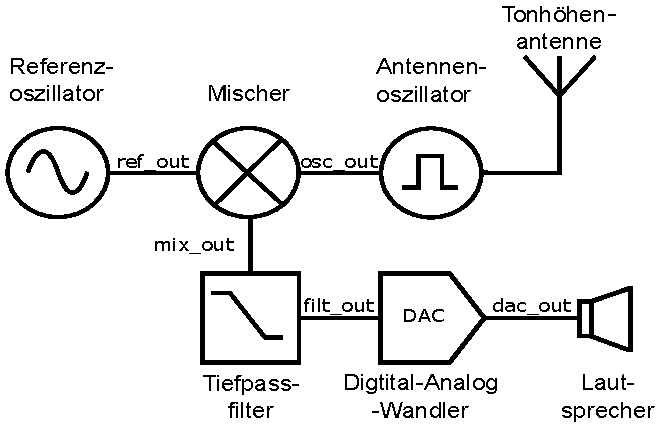
\includegraphics[width=\textwidth]{Blockschaltbild_digital.pdf}
	\caption{Blockschaltbild des digitalen Theremins}
	\label{img:Blockschaltbild_digital}
\end{figure}



\clearpage
\section{Realisierung}\label{sec:Realisierung}

Das digitale Theremin ist auf dem Entwicklungsboard DE1-SoC von Terasic aufgebaut. Dieses enthält ein Cyclone V 5CSEMA5 FPGA von Intel. Weiter befindet sich auf dem Board der Audio Codec WM8731 von Wolfson für die Ausgabe an einem Lautsprecher. In Abbildung \ref{img:Blockschaltbild_top} ist der Aufbau des digitalen Theremin aufgezeigt inklusive der Peripherie ausserhalb des FPGA.\\
Das Theremin, welches im FPGA aufgebaut ist, besteht aus zwei Bereichen. Einerseits der Signalverarbeitung und Übermittlung an den Codec. Dieser besteht aus den Komponenten \textit{Lautstärken}- und \textit{Tonhöhenverarbeitung}, \textit{DC-FIFO} und dem \textit{Audioserialisierer}. Der zweite Bereich ist das Nios II System. Dieses besteht aus dem Prozessor und diversen IP Cores, welche die Kommunikation mit den Peripherien ermöglicht. Ausserhalb des FPGA befindet sich zudem das entwickelte PCB, welches die beiden Antennenoszillatoren enthält und das Spielen des Theremins ermöglicht.\\
Die Kommunikation zwischen dem Nios II Prozessor und den anderen Komponenten geschieht über das \textit{Avalon Memory Mapped Interface}. Der Prozessor agiert in dieser Kommunikation als Master und die restlichen Komponenten als Slaves. Die Übertragung der Audioinformation in der Signalverarbeitung geschieht über das \textit{Avalon Streaming Interface}. Wobei Sender als Streaming Source und Empfänger als Streaming Sink deklariert sind. Das Streaming Interface ist notwendig für den Einsatz des Dual-Clock-FIFO (DC-FIFO). Dieses übernimmt den Übergang verschiedener Clockregionen zwischen den Komponenten \textit{Tonhöhenverarbeitung} und \textit{Audioserialisierer}.\\
Die Clocks, welche zu den verschiedenen Komponenten führen sind in Abbildung \ref{img:Blockschaltbild_top} für eine bessere Übersichtlichkeit weggelassen worden. Für eine Liste aller Clock Frequenzen und deren Ziel siehe Kapitel \ref{subsec:Clock}.

\begin{figure}[h!]
	\centering
	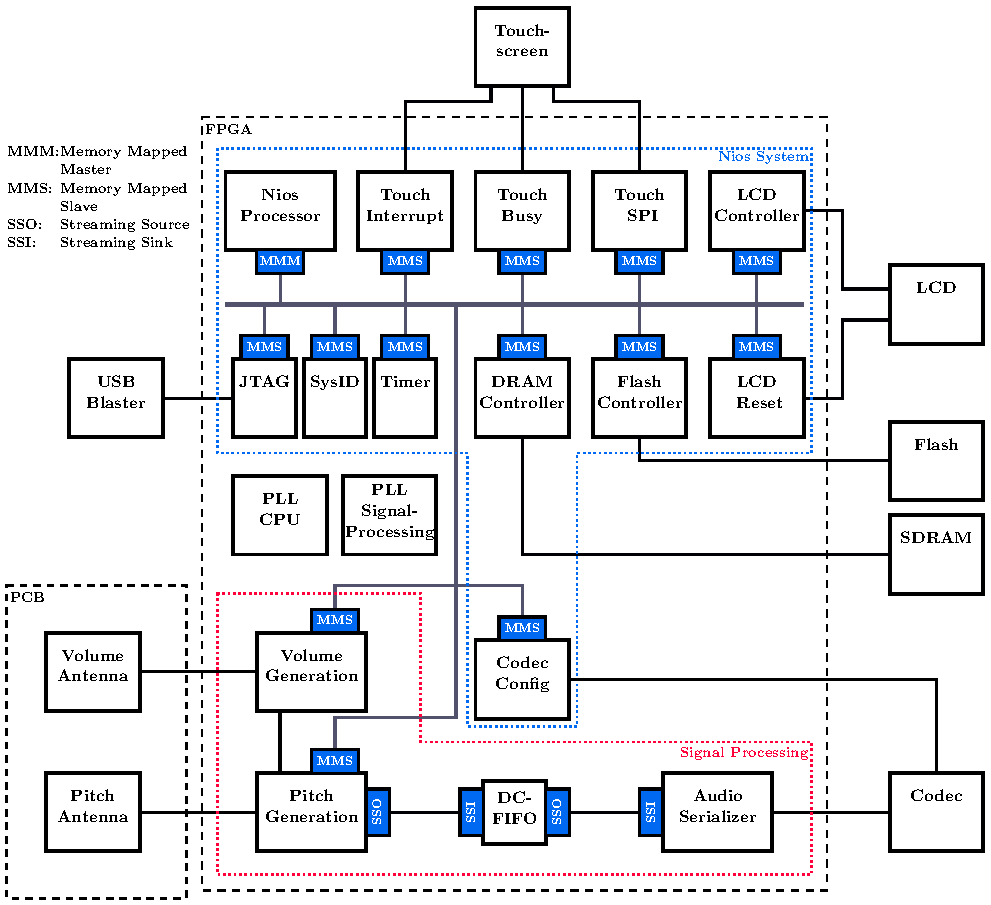
\includegraphics[width=1\textwidth]{Blockschaltbild_top.pdf}
	\caption{Blockschaltbild gesammtes Theremin} 
	\label{img:Blockschaltbild_top}
\end{figure}  

\clearpage


	\subsection{Tonhöhen- und Lautstärkenoszillator}\label{subsec:Antennenoszilator}
Für die Antennenoszillator-Schaltung haben wir uns im Projekt 5 für den Colpitts-Oszillator aus Abbildung \ref{img:colpitts} entschieden. Der Aufbau im Projekt 5 umfasste nur einen Oszillator zur Veränderung der Tonhöhe.

Es handelt sich dabei um einen Colpitts-Oszillator mit einem JFET. Diese Schaltung ist von dem Bauset ''Theremin selber bauen`` von Franzis übernommen \cite{Franzis}. 
Da der im Bauset verwendete JFET nicht mehr bestellbar ist, war ein Wechsel auf den J113 N-Kanal JFET nötig. Die mit LTspice simulierten Werte des J113 glichen stark der Originalschaltung, weshalb der Entscheid auf diesen fiel. 
Damit das Sinussignal des Antennenoszillator nicht A/D gewandelt werden muss, wandelt eine Komparatorschaltung das Sinussignal in ein Rechtecksignal mit gleicher Frequnez um. 
Diese ist mit \SI{3.3}{V} betrieben, da die Logikeingänge des FPGA auf diese Spannung ausgelegt sind. 

Im Projekt 5 wurde als Antenne ein Messingrohr verwendet. Diese ist am Anschluss pitch\_antenna verbunden. 

Die Ausgangsspannung des Colpitts-Oszillator ist über den Kondensator C11 entkoppelt. Dies entfernt den DC-Anteil. Der Kondensator C11 und die Widerstände R3 und R4 bilden zusammen einen Hochpass. Damit die Oszillatorfrequenz von ca \SI{562}{kHz} das Filter passieren kann, ist C11 so gewählt, dass die Grenzfrequenz des Filters bei ca \SI{265}{kHz} liegt. 

Auf dem PCB sind nun im Projekt 6 zwei solche Oszillatoren verbaut: Der Tonhöhenoszillator und der Lautstärkenoszillator. Das PCB ist mit einem \SI{12} {VDC} Schaltnetzteil gespiessen. Der MC7809 Spannungsregler generiert die \SI{9} {VDC} für die Colpitts-Oszillatorschaltungen. Die \SI{3.3} {VDC} für den Komperator erzeugt der LT1117 Spannungsregler. Bei der Wahl der Spannungsregler ist darauf geachtet worden, dass die erzeugten Spannungen möglichst störungsfrei ist und wenig Ripple aufwiesen. Das gesamte Schema der Schaltung ist im Anhang enthalten.

\begin{figure}[h]
	\centering
	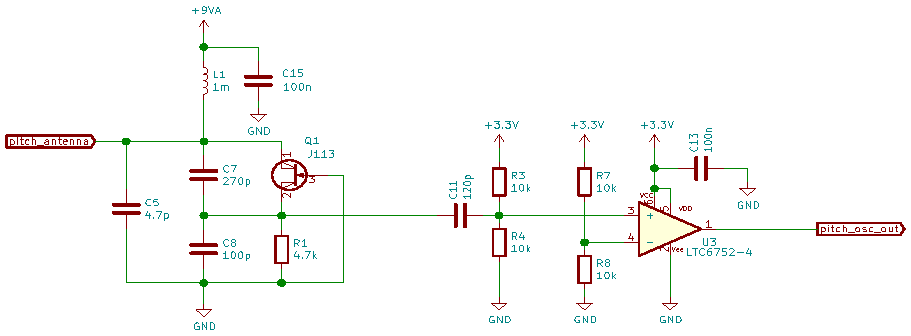
\includegraphics[width=\textwidth]{colpitts.pdf}
	\caption{Schema Antennenoszillator. Links Collpitts-Oszillator, rechts Komparatorschaltung}
	\label{img:colpitts}
\end{figure} 

\clearpage



	\subsection{Clock}\label{subsec:Clock}
Die verschiednen Clocks für die Hardwarekomponenten und die CPU werden in zwei PLL Blöcken generiert. Ein Block für die Signalverarbeitung und einer für das Nios System. In Tabelle ... \todo{Referenz einfügen} sind alle Frequenzen aufgelistet. 

\todo{Tabelle mit allen Frequenzen einfügen}


	\subsection{Nios II System}\label{subsec:CPU}
Der eingesetzte Nios II Prozessor ist für die Bedienung des Theremin und die Steuerung der Signalverarbeitungshardware zuständig. Die diversen eingesetzten IP Cores sind in den unten stehenden Kapiteln beschrieben.

\paragraph{JTAG, Timer und System ID}\mbox{}\\

Der JTAG IP Core ermöglicht das flüchtige Programmieren des Nios II wie auch das Kommunizieren mit selbem für Debugging Zwecke. 
Durch den Einsatz des Timer IP Cores erhält der Nios II einen Interval Timer, um beispielsweise periodisch Interrupts zu generieren. 
Im System ID IP Core ist die Systemidentifikationsnummer gespeichert. Diese ist nötig, um beim Laden der Software sicherzustellen, dass das passende Hardware Image vorhanden ist.
Alle drei Komponenten sind mit Standardeinstellungen in das Nios II System eingefügt worden.

\paragraph{Speicher}\mbox{}\\

Der Arbeitsspeicher ist ein externer 64MB SDRAM Chip IS42S16320D von ISSI. Für die Kommunikation mit dem Nios II Prozessor ist der SDRAM Controller IP Core zuständig. Der Nios II Prozessor kann über das Memory Mapped Interface mit dem Core kommunizieren und so auf das SDRAM zugreifen. Da dieser Chip bereits auf dem Entwicklungsboard vorhanden ist und um Ressourcen zu sparen, haben wir uns gegen On-Chip Speicher entschieden.\\

Das Hardware Image und der Programmcode sind auf dem Board enthaltenen Flash Speicher gespeichert. Dabei lädt Quartus, anders als bei dem nicht flüchtigen Programmieren, nicht das SRAM Object File (.sof) sondern ein JTAG Indirect Configuration File (.jic). Das Erstellen dieses Files geschieht im Quartus aus dem SRAM Object File und dem in Eclipse generierten HEX File. Der USB Blaster lädt das .jic File über ein Serial Flash Loader Image auf den Flash Speicher. Das FPGA kopiert beim Einschalten des Gerätes zuerst das Hardwareimage und anschliessend den Programmcode. Auf Empfehlung von Dokumentationen von Intel haben wir uns entschlossen, den Programmcode durch einen Bootcopier ins SDRAM zu kopieren. Abbildung \ref{img:FlashLayout} zeigt das Layout des Flash Speichers nach dem Programmieren \cite{non_volatile}.

\begin{figure}[h!]
	\centering
	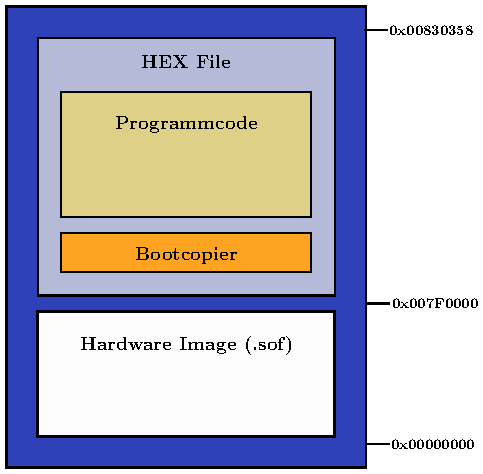
\includegraphics[width=0.45\textwidth]{FlashLayout.pdf}
	\caption{Layout des Flash Speichers} 
	\label{img:FlashLayout}
\end{figure}  

\paragraph{LCD Controller \& Reset}\mbox{}\\

Für das beschreiben des LCD ist die von Terasic bereitgestellte VHDL Komponente\\ LT24\_Controller zuständig. Der Nios II Prozessor steuert diese über das Memory Mapped Interface. Das verwendete Display LT24 von Terasic enthält für das Schreiben des LCD den LCD Treiber ILI9341 von ILITEK. Dieser Chip wird durch den LT24\_Controller über das parallele \SI{16}{Bit} Interface gesteuert. Weiter kann der LCD Chip über den PIO Core LCD Reset zurückgesetzt werden. Wie diese beiden Komponenten in Software angesteuert werden ist in Kapitel \ref{subsec:drivers} genauer beschrieben \cite{LCD_Chip}.

\newpage

\paragraph{Touchscreen}\mbox{}\\

Der Touch Screen Digitizer AD7843 von Analog Devices misst den resistiven Touchscreen des LCD aus und übermittelt die digitalisierten Koordinaten über SPI an den Prozessor. Der Nios II kommuniziert dabei über drei verschiedene IP Cores mit diesem Chip: Der SPI Core \textit{Touch SPI} für die Datenübertragung, der PIO Core \textit{Touch Busy} um den Beschäftigungsstatus des Chips abzufragen und den zweiten PIO Core \textit{Touch Interrupt}, welcher den Nios II über eine Betätigung des Touchscreens informiert. Bei einer Berührung des Touchscreens löst \textit{Touch Interrupt} beim Nios II Prozessor einen Interrupt aus, welcher sofort die Koordinaten über SPI anfordert \cite{Touch_ADC}.
	\subsection{Tonhöhenverarbeitung}\label{subsec:Pitch_Generation}

Die Hauptaufgabe der Komponente \textit{Tonhöhenverarbeitung} ist es das Audiosignal aus dem Rechtecksignal des Tonhöhenoszillators zu generieren. Die \textit{Tonhöhenverarbeitung} nimmt zudem eine Frequenzmessung des Audiosignals vor um diverse Funktionalitäten zu gewährleisten. In Abbildung \ref{img:Blockschaltbild_pitch} ist der Grobe Aufbau der Komponente aufgezeigt. Die genaue Erklärung zu den einzelnen Komponenten ist in den folgenden Abschnitten zu finden.


\begin{figure}[h!]
	\centering
	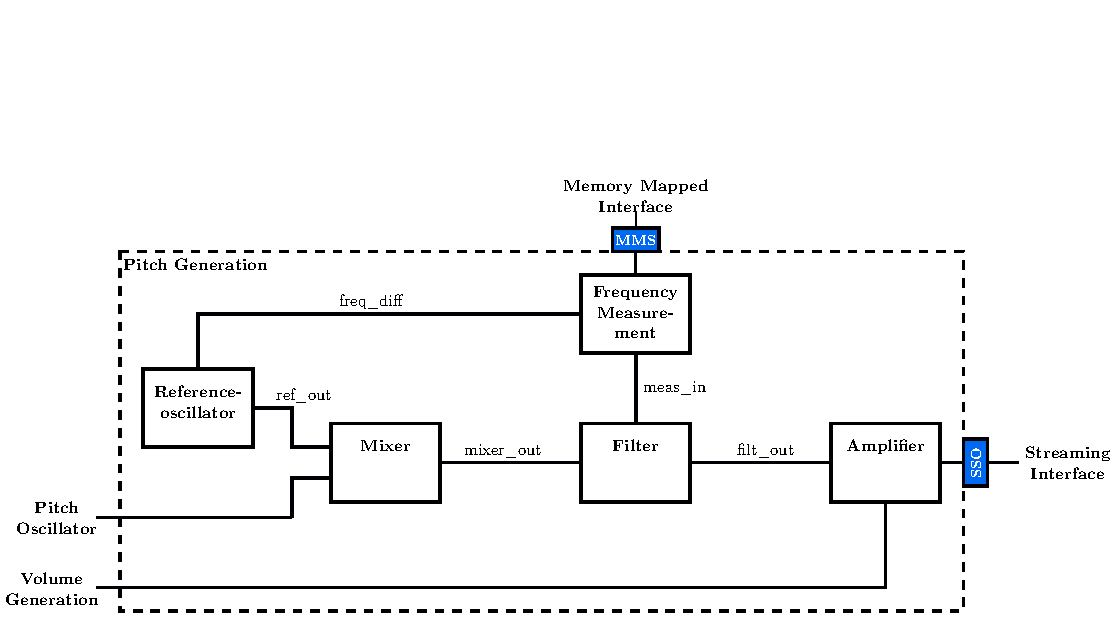
\includegraphics[width=\textwidth]{Blockschaltbild_pitch.pdf}
	\caption{Blockschaltbild der Custom IP \textit{Tonhöhenverarbeitung}} 
	\label{img:Blockschaltbild_pitch}
\end{figure}  



\paragraph{Referenzoszillator}\mbox{}\\

Der \textit{Referenzoszillator} ist wie in der analogen Version aus Kapitel \ref{subsec:Theremin_analog} dafür zuständig ein Sinussignal mit einer Frequenz nahe der des Tonhöhenoszillators zu generieren und an \textit{ref\_out} auszugeben. Er generiert diesen wie schon erwähnt mithilfe des Cordic Algorithmus. Er ist aufgeteilt in zwei Komponenten: der \textit{Cordic Prozessor} und der \textit{Cordic Controller}. Wie diese beiden Komponenten miteinander verbunden sind ist in Abbildung \ref{img:Referenceoscillator} ersichtlich. Beide Komponenten stammen aus dem Projekt 5. Änderungen, welche im Projekt 6 stattfanden, sind entsprechend gekennzeichnet. \\

\begin{figure}[t]
	\centering
	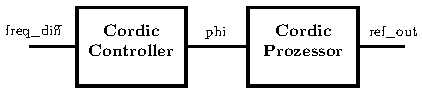
\includegraphics[width=0.53\textwidth]{Referenceoscillator.pdf}
	\caption{Aufbau des Referenzoszillators} 
	\label{img:Referenceoscillator}
\end{figure}  

Der \textit{Cordic Prozessor} ist die eigentliche Implementierung des Cordic Algorithmus wie er in Kapitel \ref{subsec:Cordic} beschrieben wurde. Er muss jedoch für den Einsatz im FPGA leicht angepasst werden. \\
Die Berechnung der Werte für \(\arctan{2^{-i}}\) fand vorgängig statt und ist in eine Lookup Table gespeichert. Dies spart Ressourcen für diese komplizierte Berechnung ein. Wir haben uns entschieden den Algorithmus in einer Pipeline zu implementieren. Dies führt einerseits zu einer höheren maximalen Clockfrequenz, andererseits aber auch zu einer grösseren Signallatenz. Dies ist jedoch nicht problematisch für die gewählte Anwendung, da die Latenz im Nanosekundenbereich ist und später nicht hörbar auffällt. Zuletzt ist eine Multiplikation mit \(2^{-i}\) ganz einfach durch eine Verschiebung um \(i\) Bits nach rechts ersetzbar. Dies spart wiederum Ressourcen ein.\\
Das berechnete Resultat ist als signed Zahl definiert um die Berechnung von negativen Zahlen zu ermöglichen. Sie sind im fixed-point Format und haben \SI{16}{Bit} Länge. Dabei sind von den \SI{16}{Bit} \SI{1}{Bit} Vorzeichen und \SI{15}{Bit} Nachkommastellen. Dies entspricht einem Zahlenbereich von -1 bis 0.999969. Die berechneten Werte gibt der \textit{Cordic Prozessor} an \textit{ref\_out} aus.

Für die Berechnung der Sinuswerte muss ein Winkelwert berechnet werden, der mit der Zeit so ändert, dass sich am Ausgang des Cordic Prozessor ein Sinus mit der gewünschten Frequenz ergibt. Der berechnete Winkelwert wird an \textit{phi} ausgegeben. Für diese Aufgabe ist der \textit{Cordic Controller} zuständig. Bei mit der Zeit linear ansteigendem Winkelwert ergibt sich am Ausgang die gewünschte Sinusform. Wichtig ist jedoch, dass der Cordic Algorithmus nur für Winkelwerte zwischen \(-\pi/2\) und \(\pi/2\) oder anders für Werte im ersten und zweiten Quadranten konvergiert. Die Lösung für dieses Problem ist in Abbildung \ref{img:Cordic_phi} ersichtlich. 
Als erstes wird der Sägezahn Winkel berechnet. Für den linearen Anstieg des Winkels zählt der \textit{Cordic Controller} einen Zähler mit einer bestimmten Schrittweite jeden Clockzyklus hoch. Der wrap-around des Zählers ist dabei erwünscht um den Sprung zwischen dem II und III Quadranten zu erzielen. Der Schrittwert ergibt sich wie folgt:

\begin{equation}
step = \frac{2^{n+1}f_{sig}}{f_{clk}}
\label{equ:cordic_step}
\end{equation} 

Wobei \(n\) die Anzahl Bits des Wertebereichs des Dreiecks Winkels ist, \(f_{sig}\) die gewünschte Frequenz des generierten Signals und \(f_{clk}\) die Clock Frequenz des FPGA.

Nun kommt die bereits erwähnte Einschränkung des Cordic Algorithmus ins Spiel. Die berechneten Werte des Sägezahnwinkels zwischen dem II und III Quadranten konvergieren nicht. Aus diesem Grund konvertiert der \textit{Cordic Controller} diesen Winkel in den Dreieckswinkel. Sind die beiden vordersten Bits entweder \(01\) oder \(10\) befindet sich der Winkelwert im II respektive III Quadranten. Um in diesem Fall den Dreieckswinkel zu erhalten invertiert der \textit{Cordic Controller} alle Bits ausser dem most-significant Bit. Wie man sich leicht davon überzeugen kann ergibt der Dreieckswinkel denselben Sinusverlauf wie der Sägezahnwinkel bei einer Sinusrechnung ohne die erwähnten Einschränkungen. \cite{Cordic}

Um die Kalibrierung und den Glissandoeffekt für das Theremin zu ermöglichen waren im Projekt 6 kleine Anpassungen am \textit{Cordic Controller} nötig. Wie zuvor hat der Controller eine fixe Frequenz implementiert, welche in der Grössenordnung \SI{550}{kHz} liegt. Jedoch legt die Frequenzmessungskomponente nun eine Differenz über einen Eingang an den Cordic Controller an um die zuvor genannten Features über den Referenzoszillator zu ermöglichen.


\begin{figure}[t]
	\centering
	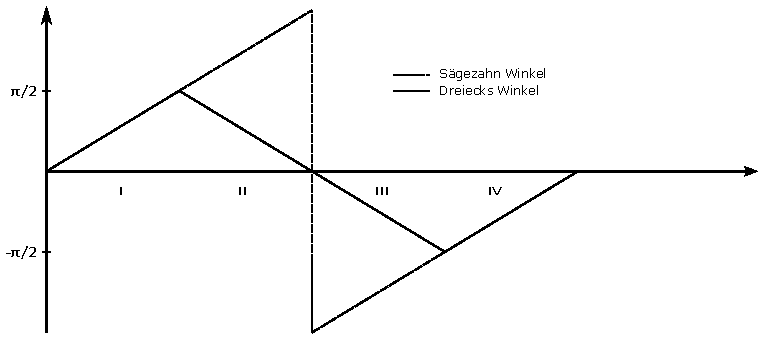
\includegraphics[width=0.8\textwidth]{Cordic_phi.pdf}
	\caption{berechneter Winkel \textit{phi} des Cordic Controllers in Funktion der Zeit} 
	\label{img:Cordic_phi}
\end{figure}  


\paragraph{Mischer}\mbox{}\\

Die Implementation des \textit{Mischers} ist dank der Entscheidung für die Rechteckform des Tonhöhenoszillatorsignals sehr einfach. Über einen GPIO liest der Mischer das Signal des Tonhöhenoszillators ein und verrechnet es mit dem generierten Sinus \textit{ref\_out}. Eine \textit{1} des Rechtecks wird dabei als die Zahl \textit{1} und eine \textit{0} als die Zahl \textit{-1} interpretiert. Die Multiplikation zwischen der \textit{1} und \textit{ref\_out} ist dabei nicht nötig und eine Multiplikation mit \textit{-1} erzielt der Mischer durch das Bilden des Zweierkomplement von \textit{ref\_out}.

\paragraph{Filter}\mbox{}\\

Im Projekt 5 war das \textit{Filter} ein einzelnes CIC-Filter mit dem Dezimationsfaktor 1000. Dies hatte zur Folge, dass viel Aliasing entstand. Um dieses zu verringern haben wir uns im Projekt 6 für den Aufbau aus Abbildung \ref{img:Filter_Pitch} entschieden. Die drei Filter CIC 1 bis CIC 3 sind Instanzen einer CIC-Filter Komponente. Diese Komponente stammt weitestgehend aus dem Projekt 5, ist jedoch auf mehr Modularität erweitert. Die Parameter der drei Instanzen sind in Tabelle \ref{tab:cic_pitch} ersichtlich. Da es bei CIC-Filtern wie in Kapitel \ref{subsec:CIC_Filter} beschrieben, um deren Nullstellen zu Aliasing kommt, sind diese Filter so eingestellt, dass sich die Oberwellen des Rechteck möglichst nicht in deren Nähe befinden. Bei \textit{CIC 1} wurde eine höhere Ordnung gewählt um am Anfang eine stärkere Dämpfung zu erzielen. Die Anzahl Ausgangsbits erhält man mit Formel \ref{equ:cic_bitgrowth} in Kapitel \ref{subsec:CIC_Filter}.\\
Zuletzt haben wir noch ein FIR-Filter implementiert um das Signal auf 48kHz unter abzutasten. Das Filter hat eine Passfrequenz von \SI{2}{kHz} und eine Stopfrequenz von \SI{24}{kHz} mit einer Dämpfung von 55dB. Wir entschieden uns die Koeffizienten mit dem \textit{filterDesigner Tool} von Matlab zu berechnen und als \SI{27}{Bit} signed Zahlen in einer Lookup Table zu speichern. Wir wählten deshalb \SI{27}{Bit}, da im FPGA eine solche Multiplikation noch knapp in einen DSP Block integriert werden kann. \cite{Cyclone_V}
Weswegen der Ausgang Frequenzmessung nach dem zweiten CIC-Filter gewählt wurde ist in einem späteren Abschnitt beschrieben.


\begin{figure}[t]
	\centering
	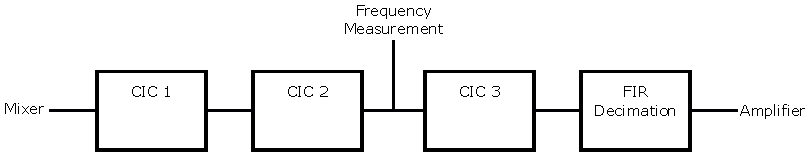
\includegraphics[width=1\textwidth]{Filter_pitch.pdf}
	\caption{Aufbau des Filters in der Komponente Pitch Generation} 
	\label{img:Filter_Pitch}
\end{figure}  

\begin{table}[t]
	\centering
	\caption{Parameter der drei CIC-Filter}
	\label{tab:cic_pitch}
	\begin{tabular}{l|l|l|l|l}
		\textbf{Komponente} & \textbf{Dezim.Fakt.} & \textbf{Ordnung} &  \textbf{Ausgangsfreq.} & \textbf{Ausgangsbits}\\
		\hline\hline
		CIC 1 & 5 & 2 & \SI{10.8}{MHz} & \SI{21}{Bits}  \\ \hline
		CIC 2 & 9 & 1  & \SI{12}{MHz} & \SI{25}{Bits}  \\ \hline
		CIC 3 & 5 & 1 & \SI{240}{kHz} & \SI{28}{Bits}  \\ \hline	
	\end{tabular}
\end{table}

\paragraph{Verstärker}\mbox{}\\

Die Komponente \textit{Verstärker} ist dafür zuständig beim Signal \textit{filt\_out} den Gain der CIC-Filter zu kompensieren und anschliessend dieses mit der Dämpfung, welche die Lautstärkeverarbeitung liefert, zu multiplizieren. In Abbildung \ref{img:Zero_Cross} ist eine Problematik aufgezeigt, welche auftritt, wenn man die Dämpfung zu beliebigen Zeiten wechselt. Links ist zu sehe, was passiert, wenn die Dämpfung beim höchsten Wert der positiven Halbwelle ändert. Diese Sprünge im Signal treten dann als hörbares Knacksen auf. Um dies zu verhindern ist eine Erkennung von Nulldurchgängen implementiert, dass wie in der Abbildung rechts die Dämpfungen nur bei diesen Nullstellen ändern. Da der Codec ein offsetbehaftetes Signal verlangt muss das most-significant Bit des Signal getoggelt werden um dies zu bewerkstelligen. Diese Komponente enthält zudem die Kommunikation mit dem Streaming Interface. \\
Die Dämpfung des Audiosignals könnte auch über den Codec gemacht werden. Weshalb dies nicht möglich ist, ist in Kapitel \ref{subsec:audio} beschrieben. 
	
\begin{figure}[h!]
	\centering
	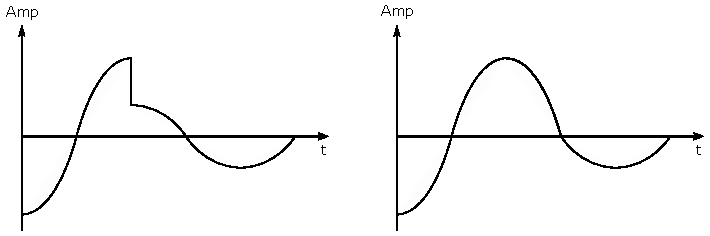
\includegraphics[width=1\textwidth]{Zero_Cross.pdf}
	\caption{Unterschied Dämpfungswechsel (links ohne und rechts mit Nullstellenerkennung)} 
	\label{img:Zero_Cross}
\end{figure}  

\newpage

\paragraph{Frequenzmessung, Kalibration \& Glissandoeffekt}\mbox{}\\

Die Komponente \textit{Frequenzmessung} hat mehrere Aufgaben und ist diejenige Komponente mit welcher über den Nios II Prozessor die gesamte \textit{Tonhöhenverabreitung} gesteuert werden kann. Der Aufbau dieser Komponente ist in Abbildung \ref{img:freq_meas_pitch} aufgezeigt.\\
Zum einen wird hier die Frequenzmessung durchgeführt. Dies geschieht über die drei Komponenten FIR, Periodenzähler und Goldschmidtdividierer. FIR ist wie der Name sagt ein FIR Filter. Dieses ist nötig um das Signal aus den CIC-Filtern, welches noch hochfrequente Anteile enthält zu filtern. Das FIR Filter hat eine Passfrequenz von \SI{2}{kHz} eine Stopfrequenz von \SI{40}{kHz} und eine Dämpfung von 30dB. Das Filter ist mit dem \textit{filterDesigner} Tool in Matlab berechnet. Wir haben entschieden die Filterkoeffizienten als fixed-point signed Zahlen in einem Array mit \SI{18}{bit} länge abzuspeichern. Auf dieser Koeffizientenlänge kann Quartus die DSP-Blöcke so nutzen, dass nach der Multiplikation des Signals mit den Koeffizienten die Resultate gleich in den Blöcken addiert wird. Dies ermöglicht längere Multiplikationsketten. \cite{Cyclone_V}\\
Anschliessend wird das Signal \textit{fir\_out} im \textit{Periodenzähler} ausgemessen. Dieser zählt von Nulldurchgang zu Nulldurchgang einen Zähler hoch. Bei einem Nulldurchgang wird der Wert dieses Zählers am Signal \textit{per\_cnt} ausgegeben. Der Zählerwert entspricht der Anzahl Abtastwerte des Signals in einer Signalperiode. \\
Das Signal hat eine Abtastfrequenz von \SI{1.2}{MHz}. Dividiert man diese Abtastfrequenz durch die zuvor gezählte Anzahl Abtastperioden erhält man die Frequenz des Signals.\\ Um diese Division zu berechnen haben wir uns entschieden den Goldschmidt Algorithmus aus Kapitel \ref{subsec:Goldschmidt} einzusetzen. Dieser hat den Vorteil, dass er auch Nachkommastellen berechnen kann um die nötige Genauigkeit bei den tiefen Frequenzen zu erreichen wie in Kapitel \ref{subsec:Musiktheorie} beschrieben. Dass die Berechnungsdauer des Algorithmus nicht für alle Zahlen gleich ist, ist nicht Problematisch, da diese Zeiten im Nanosekundenbereich liegen und nicht hörbar sind. Der Messbereich der Frequenzmessung fängt bei \SI{100}{Hz} an und geht bis \SI{10}{kHz}. Alle Frequenzen darunter oder darüber zeigen \SI{100}{Hz} respektive \SI{10}{kHz} an.

\begin{figure}[h!]
	\centering
	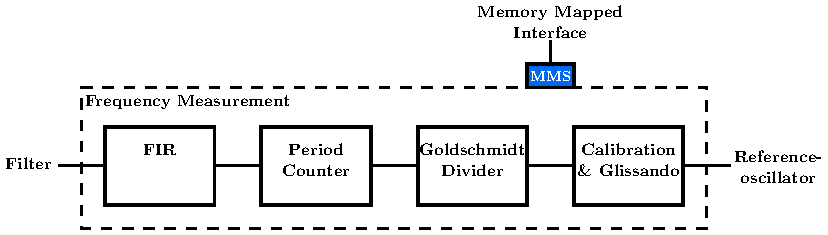
\includegraphics[width=1\textwidth]{freq_meas_pitch.pdf}
	\caption{Aufbau der Frequenzmessung, Kalibration und Glissandoeffekt in der Komponente Pitch Generation} 
	\label{img:freq_meas_pitch}
\end{figure}  

Die gemessene Frequenz wird anschliessend in der Komponente \textit{Kalibration \& Glissando} benötigt. Diese ist dafür zuständig einerseits die Tonhöhe zu kalibrieren und andererseits den Glissando-Effekt zu steuern. Um die Frequenz des Audiosignals für diese Funktionen zu verändern verstimmt die Komponente den Referenzoszillator entsprechenden. Kalibration \& Glissando addiert die Differenz welche den Glissandoeffekt hervorruft und die Änderung welche während der Kalibration berechnet wurde und übergibt das Resultat dem Referenzoszillator. Diese wird von nun an als Frequenzdifferenz bezeichnet. Die Steuerung dieser Funktionen ist als State-Machine aufgebaut wie in Abbildung \ref{img:state_event_Cal_Glis} zu sehen ist. 
Dabei sind die States reset, check, sign und diff für die Kalibration zuständig und freq range, step und step count für den Glissando-Effekt zuständig. Es folgt eine Erklärung, was in den einzelnen Zuständen geschieht:

\textbf{Idle}:
Der Idle State setzt die Frequenzdifferenz auf die berechnete Differenz der Kalibrierung. Der Anteil des Glissando-Effekts wird auf 0Hz gesetzt.

\textbf{reset}:
Der alte Kalibrationswert wird gelöscht und gewartet bis eine neue Frequenzmessung abgeschlossen ist.

\textbf{check}:
Da die Messung Frequenzen unter \SI{100}{Hz} immer als \SI{100}{Hz} angibt, muss die Komponente diese erkennen. Bei einer Messung von \SI{100}{Hz} inkrementiert die Komponente Calibration \& Glissando die Frequenzdifferenz um \SI{400}{Hz}. Dies führt dazu, dass bei der nächsten Messung das Signal nicht mehr in dem Bereich liegt, in dem die Messung immer \SI{100}{Hz} misst.

\textbf{sign}:
Für die in Kapitel \ref{sec:Konzept} beschriebene Spielweise, dass mit kleinerer Distanz zur Antenne die Tonhöhe steigt, ist der State sign zuständig. Ist der Referenzoszillator so eingestellt, dass dessen Frequenz kleiner ist als die des Tonhöhenoszillators, so würde bei Annäherung des Spielers an die Antenne die Frequenz des Audiosignals zuerst sinken, bis die beiden Oszillatorfrequenzen gleich sind. Dies, da die Frequenz des Tonhöhenoszillators mit kleinerem Abstand immer mehr sinkt. Anschliessend würde sie wieder steigen, da der Tonhöhenoszillator kleiner ist als der Referenzoszillator. Um zu erkennen ob dies der Fall ist, subtrahiert die Komponente \SI{100}{Hz} von der Frequenzdifferenz. Ist die nachfolgende Messung grösser geworden, bedeutet dies, dass der Referenzoszillator kleiner war als der Tonhöhenoszillator. Nun kann ganz einfach die gemessene Frequenz verdoppelt und zu der Frequenzdifferenz addiert werden, damit der Referenzoszillator die grössere Frequenz hat.

\textbf{diff}:
Nach den letzten drei States ist nun sichergestellt, dass der Referenzoszillator grösser ist als der Tonhöhenoszillator. Jedoch sollen ja diese beiden Oszillatoren aufeinander abgestimmt sein. Dazu wird abwechslungsweise die Frequenzdifferent um einen kleinen Schritt dekrementiert und danach die Frequenz gemessen. Wir haben uns dafür entschieden, dass wenn die Messung \SI{120}{Hz} unterschreitet die Kalibration abgeschlossen ist. Dies da Töne unterhalb dieser Frequenz sehr merkwürdig klingen.

\textbf{freq range}:
Der State freq range ist dafür zuständig herauszufinden, welcher diskrete Ton der gewählten Tonleiter (normal oder pentatonisch) am nächsten zur gemessenen Frequenz ist. Die Frequenz wird dabei mit einer Lookup-Table mit allen Grenzen zwischen den Tönen verglichen. ist die Frequenz ausserhalb des gewählten Frequenzbereich wird hier abgebrochen und in den State idle gewechselt.

\textbf{step}:
Der State step bestimmt die Schrittgrösse, welcher im nächsten State für die Annäherung nötig ist. Die Schrittgrössen für alle Töne sind im Vorhinein berechnet als \SI{1}{Cent} Differenz zum eigentlichen Ton. Würde überall die gleiche Schrittgrösse genommen, wäre das Aufschliessen bei hohen Tönen extrem langsam und bei tiefen Tönen so schnell, dass kein Übergang hörbar ist. 

\textbf{step count}:
Der letzte State verrechnet die Frequenzdifferenz in vorgegebenen Intervallen mit dem zuvor bestimmten Step, bis auf den Ton aufgeschlossen ist. Hat die Frequenzmessung jedoch während dem Zählen eine neue Frequenz gemessen wird in den State freq range gewechselt. Erreicht das Aufschliessen bevor eine neue Messung stattfand einen Unterschied von unter \SI{6}{Cent} zu der anzunähernden Frequenz, stoppt das Zählen bis zu einer neuen Messung.

\begin{figure}[h!]
	\centering
	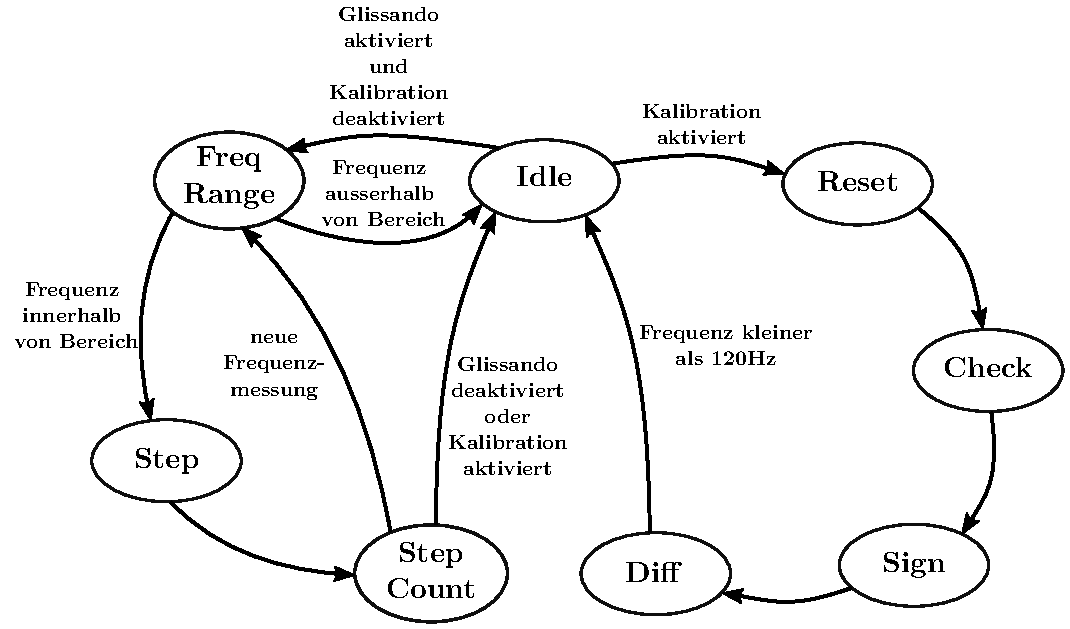
\includegraphics[width=1\textwidth]{state_machine_Cal_Glis.pdf}
	\caption{State Event Diagramm der Kalibration \& Glissando Komponente} 
	\label{img:state_event_Cal_Glis}
\end{figure} 

\paragraph{Register}\mbox{}\\
Um mit der Komponente \textit{Tonhöhenverarbeitung} über das Memory-Mapped Interface kommunizieren zu können haben wir folgende Register definiert:

\begin{table}[H]
	\centering
	\caption{Zusammenfassung der Register}
	\label{tab:Registers_pitch}
	\begin{tabular}{l|l|l|l|l|l|l}
		\textbf{Register} & \textbf{Adresse} & \textbf{R/W} &	\multicolumn{4}{l}{\textbf{Bits}} \\\cline{4-7}
						  &					 &				& \textbf{31-3}  & \textbf{2} & \textbf{1} & \textbf{0}\\ 
		\hline \hline
		
		cntrl\_reg & 00 & R/W & X & scale & cal & glis \\ 
		\hline
		freq\_data\_reg & 01 & R & \multicolumn{4}{l}{Frequenz} \\
		\hline
		delay\_data\_reg & 10 & W & \multicolumn{4}{l}{Verzögerung} \\
	\end{tabular}
\end{table}

\begin{table}[H]
	\centering
	\caption{Control Register Flags}
	\label{tab:Register_pitch_cntrl}
	\begin{tabular}{l|l|l|l}
		\textbf{Bits} & \textbf{Kürzel} & \textbf{R/W} &	\textbf{Beschreibung}\\
		\hline \hline
		
		0 & glis & W &  1 = Glissando-Effekt aktiviert \\ 
		  &      &   &  0 = Glissando-Effekt deaktiviert \\ 
		\hline
		1 & cal & R/W &  1 = Kalibration aktiviert \\ 
		  &     &     &  0 = Kalibration beendet \\ 
		\hline
		2 & scale & W &  1 = Pentatonische Tonleiter \\ 
		 &     &       &  0 = Normale Tonleiter \\ 
		\hline

	\end{tabular}
\end{table}

Das Register \textit{freq\_data\_reg} enthält die Frequenz für die Anzeige der Spielgenauigkeit. Mehr dazu in Kapitel \ref{subsec:audio}. \\
Das Register \textit{delay\_data\_reg} enthält die Einstellung für die Zeit, die der Glissando-Effekt benötigt um die Töne zu korrigieren. Es können Werte von 0 bis 9 geschrieben werden um diese Zeit zu verändern.


	\subsection{Volume Generation}\label{subsec:Volume_Generation}
bla bla



	
\subsection{Audioserialisierer}\label{subsec:Audio_Serializer}

Für die Übertragung der Audiodaten zum Codec ist der \textit{Audioserialisierer} zuständig. Obwohl es von Intel bereits eine IP gäbe, um diese Übertragung zu übernehmen, mussten wir diese Komponente nochmals selber schreiben. Der zur Verfügung gestellte IP Core benötigt eine spezifische Clockfrequenz von \SI{12.288}{MHz}. Jedoch müssen die Tonhöhenverarbeitung und der Serialisierer Clocks erhalten, die denselben Referenzclock besitzen, um nicht Daten zu verlieren. Die verlangten Clockfrequenzen von \SI{54}{MHz} für die Tonhöhenverarbeitung und die zuvor genannten \SI{12.288}{MHz} können nicht in einem PLL generiert werden. \\
Wie der Name der Komponente schon sagt, serialisiert sie die parallelen Daten für die Übertragung. Dabei sieht der geforderte Signalverlauf des Codec wie in Abbildung \ref{img:Codec_Signals} dargestellt aus. Der Audioserialisierer gibt jeweils für den linken und rechten Kanal dieselben Daten aus. Die Signale DACLRC und BCLK werden vom Codec nach der Konfiguration, beschrieben in Kapitel \ref{subsec:audio}, vom Codec generiert und sind Eingänge des Audioserialisierers. Bei jeder positiven Flanke von DACLRC lädt der Serialisierer einen neuen Audiosignalwert ins Schieberegister und schiebt bei jeder negativen Flanke des BCLK ein neues Bit ins Signal DACDAT.

Die Komponente Audioserialisierer ist in der Datei \textit{audio\_serializer.vhd} zu finden.

\begin{figure}[t]
	\centering
	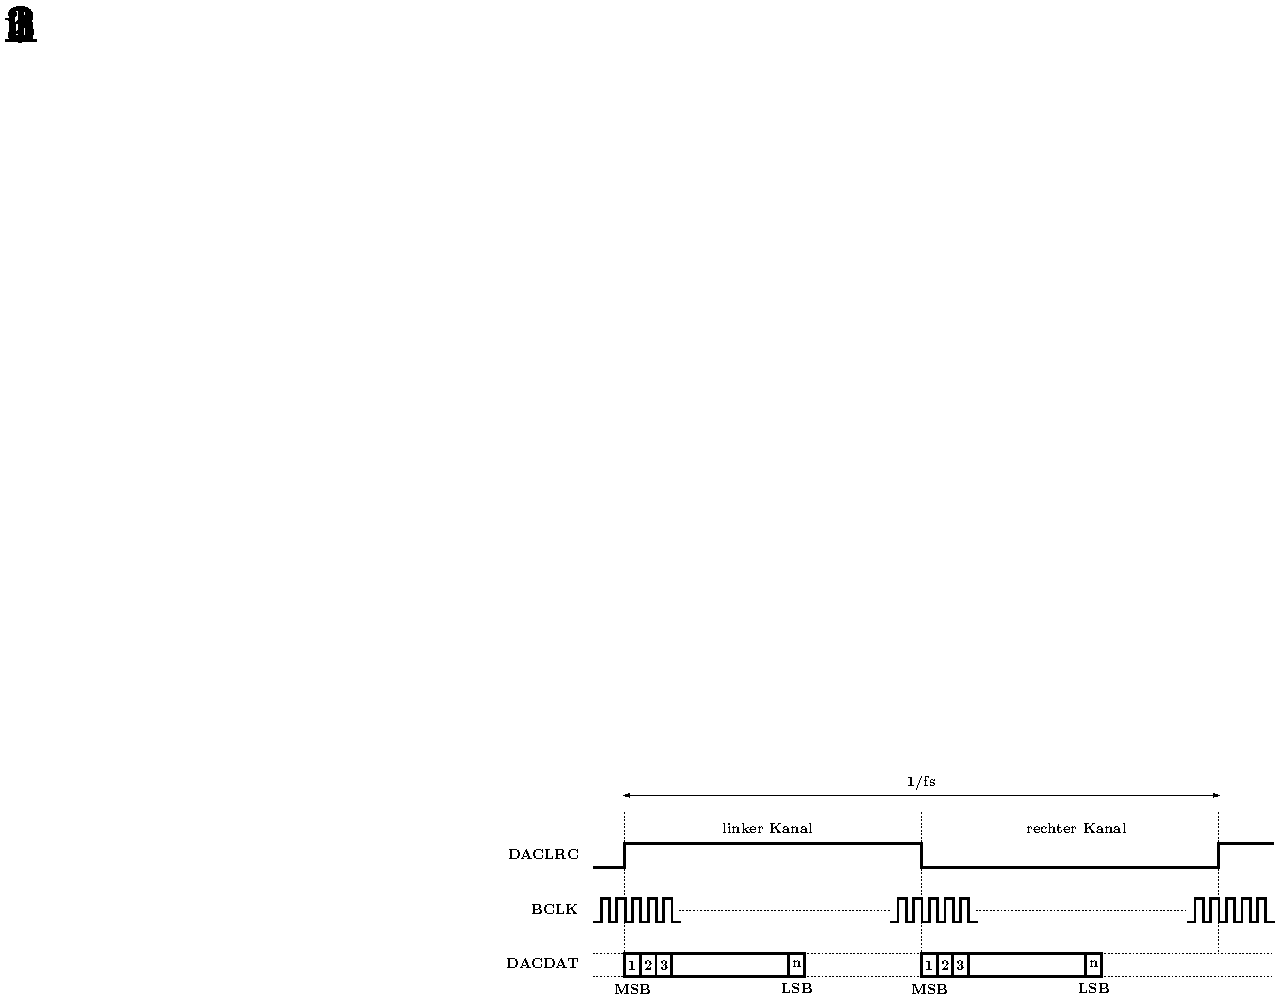
\includegraphics[width=\textwidth]{Codec_Signals_Serializer.pdf}
	\caption{Signalverlauf des Codec Interface} 
	\label{img:Codec_Signals}
\end{figure}  
	\newpage
\subsection{Lizenzen}\label{subsec:Lizenzen Hardware}
In Tabelle \ref {tab:Verwendete_IP} sind die verwendeten Intellectual Property (IP) Cores und deren Hersteller aufgelistet.
\begin{table}[H]
	\centering
	\caption{Verwendete IP}
	\label{tab:Verwendete_IP}
	\begin{tabular}{l|l}
		\textbf{Bezeichnung IP} & \textbf{Hersteller}	\\
		\hline \hline
		
		PLL  & Intel   \\ 
		\hline
		Nios II  & Intel   \\ 
		\hline
			JTAG  & Intel   \\ 
		\hline
				Timer  & Intel   \\ 
		\hline
				Sysid		  & Intel   \\ 
		\hline
					Dram Controller		  & Intel   \\ 
		\hline
					 SPI Core		  & Intel   \\ 
		\hline
					Audio and Video Config		  & Intel   \\ 
		\hline
							Flash Controller		  & Intel   \\ 
		\hline
							PIO Core		  & Intel   \\ 
		\hline
		LT24 Controller  &  Terasic  \\ 
		\hline
	
	\end{tabular}
\end{table} 



\pagebreak

\clearpage
\section{Realisierung Software}\label{sec:Realisierung_Software}
Im folgenden Teil des Fachberichtes ist der Aufbau der Software beschrieben. Es folgt zu Beginn eine Gesamtübersicht.

Die Software ermöglicht die Bedienung des Theremin. Zur Steuerung des Theremin ist auf dem Nios II eine in C programmierte State Machine realisiert. Die Bedienung geschieht über das LT24 LCD Touch Modul von Terasic. Die von Terasic zur Verfügung gestellten C Dateien zur Ansteuerung des LCD und des Touch, sowie die Dateien zur Darstellung des GUI, stellten sich als wenig brauchbar heraus. Die darin enthaltenen Funktionen sind oft zu ineffizient. Daher entschieden wir uns diese Funktionen selber zu schreiben.
	\subsection{Hauptprogramm State Machine}\label{subsec:State_Machine}
Abbildung \ref{img:state_machine} zeigt links die Initialisierung und rechts den Hauptprogrammfluss der Software als State Machine.
\begin{figure}[h]
	\centering
	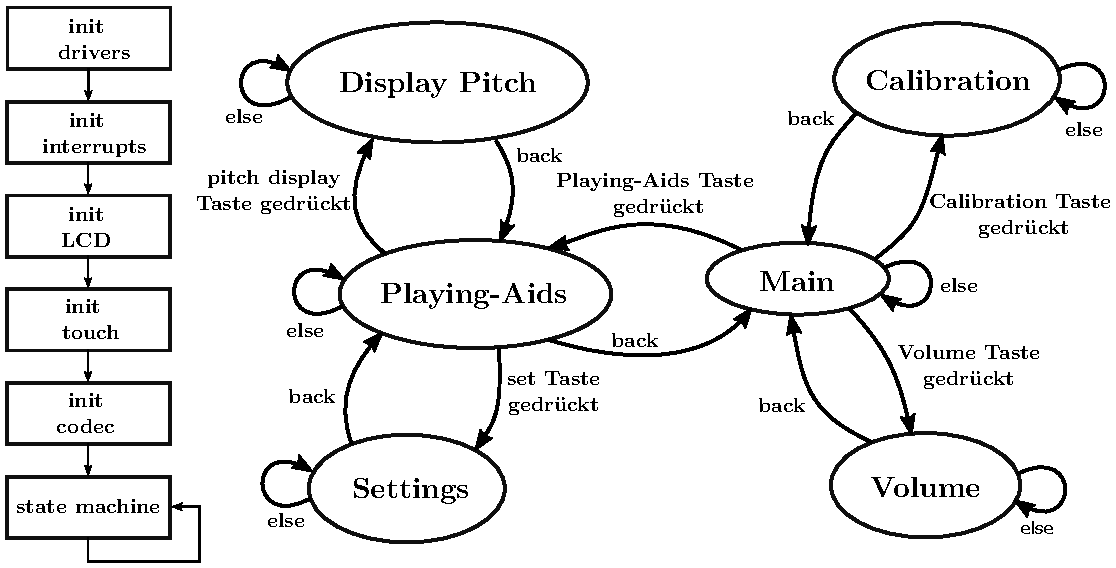
\includegraphics[width=\textwidth]{state_machine.pdf}
	\caption{State Machine und Initailisierung.}
	\label{img:state_machine}
\end{figure}

Als erstes initialisiert das Programm alle Treiber, den Touchscreen, das LCD, und den Codec. Anschliessend führt das Programm in einer Endlosschlaufe die State Machine aus. Es folgen kurze Erklärungen zu jedem State.

\textbf{Main}:
Dies ist der erste State nachdem Initialisierungsvorgang. Der Main State wartet auf eine Betätigung der drei in Abbildung \ref{img:main_screen} gezeigten Tastern. Eine Betätigung der drei Tastern führt zu einem Wechsel in den entsprechenden State. 
 
\textbf{Calibration}:
Der Calibration State fordert den Benutzer auf seine rechte Hand in die Nähe der rechten Antenne zu halten.
Nach zwei Sekunden startet die Kalibrierung. Sobald die Kalibrierung abgeschlossen ist, kann der Benutzer über den \textit{back} Taster zurück in den Main State gelangen. Abbildung \ref{img:calibration_screen} zeigt die Darstellung des LCD nach erfolgreicher Kalibrierung.

\textbf{Volume}:
In diesem State kann der Benutzer die Lautstärke ändern und die Lautstärkenantenne aktivieren und deaktivieren. Die Lautstärke kann in 10 verschiedene Pegeln eingestellt werden. Dies geschieht mithilfe der in Abbildung \ref{img:vol_screen} gezeigten \textbf{\textit{+}} und \textbf{\textit{-}} Tasten. Beim betätigen der \textit{vol antenna} Taste wird die Lautstärkenantenne je nach aktuellem Zustand deaktiviert oder aktiviert. Mit dem betätigen der \textit{back} Taste gelangt der Benutzer in den Main State.
 
\textbf{Playing-Aids}:
Im State Playing Aids kann der Benutzer mit der\textit{Glissando on} Taste den Glissando-Effekt aktivieren und deaktivieren. Die Abbildungen \ref{img:play_aids_off} und \ref{img:play_aids_on} zeigen die grafische Realisierung dieser Taste. Über die \textit{Set} Taste gelangt der Benutzer in den State Settings. Durch betätigen des \textit{display pitch} Taste wird in den State Pitch Display gewechselt. Zurück in den Main State gelangt man über die \textit{back} Taste.

\textbf{Settings}:
Im Settings State können Einstellungen am Glissando-Effekt gemacht werden. Der Delay des Glissando-Effekts ist in 10 Stufen einstellbar. Zudem kann der Anwender mit dem Taster \textit{pentatonic on/off} zwischen der pentatonischen und der normalen Tonleiter wechseln. Mit dem betätigen der \textit{back} Taste gelangt der Benutzer in den Playing-Aids State. Abbildung \ref{img:settings_screen} zeigt wie der Setting State auf dem LCD aussieht.

\textbf{Pitch Display}:
Dieser State unterstützt den Theremin Spieler dabei Töne der Tonleiter zu treffen. Der Spieler bekommt über das Display eine optische Rückmeldung in welcher Region der Tonleiter sich der gespielte Ton befindet. So muss der Spieler nicht alleine auf sein Gehör vertrauen.
Abbildung \ref{img:play_help_screen} zeigt die Darstellung dieses States.  
Der Schriftzug oberhalb des LCD zeigt den Ton an, der sich in der Region der gespielten Frequenz befindet. 
Der kleine vertikale Strich zeigt dem Spieler an wie weit weg die aktuell gespielte Frequenz von dem Ton der Tonleiter ist. 
Diese graphische Unterstützung kann jedoch nur bei der pentatonischen Tonleiter angewendet werden. Da die Antenne sehr empfindlich auf Änderungen ist, ist es mit der normalen Tonleiter nicht hilfreich den vertikalen Strich anzuzeigen. Daher haben wir uns entschieden diese Anzeige nur bei der pentatonischen Tonleiter zu verwenden.

\begin{figure}[!ht]
	\subfloat[Main Menu\label{img:main_screen}]{%
		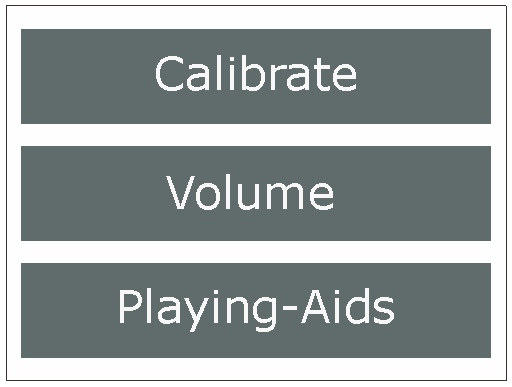
\includegraphics[width=0.3\textwidth]{Main.pdf}
	}
	\hfill
	\subfloat[Calibration Menu\label{img:calibration_screen}]{%
		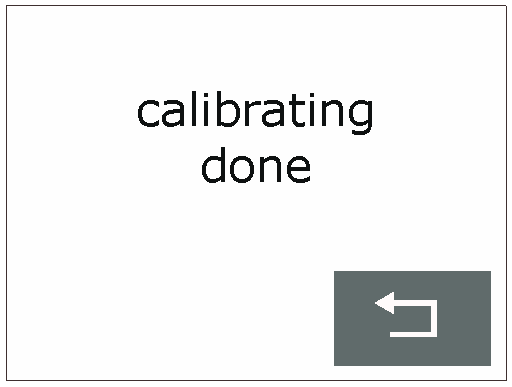
\includegraphics[width=0.3\textwidth]{calibrating_done.pdf}
	}
	\hfill
	\subfloat[Volume Menu\label{img:vol_screen}]{%
		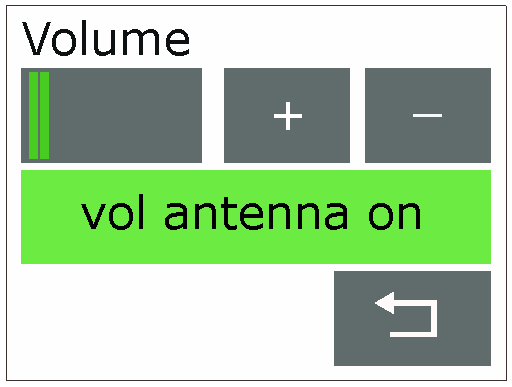
\includegraphics[width=0.3\textwidth]{volume.pdf}
	}
	\\
	\subfloat[Playing-Aids Menu, Glissando off\label{img:play_aids_off}]{%
		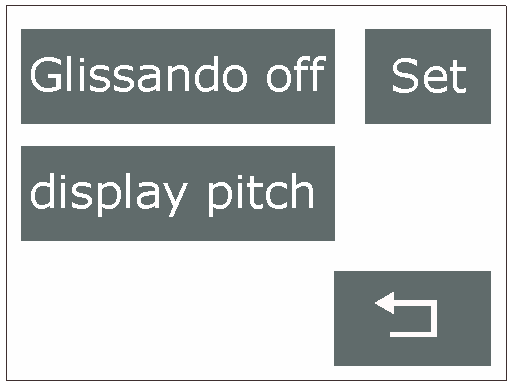
\includegraphics[width=0.3\textwidth]{play_aids.pdf}
	}
	\hfill
	\subfloat[Playing-Aids Menu, Glissando on\label{img:play_aids_on}]{%
		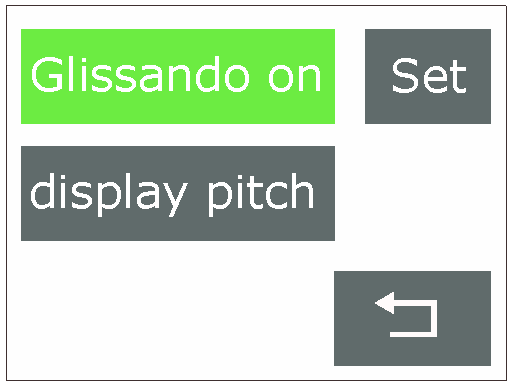
\includegraphics[width=0.3\textwidth]{play_aids_on.pdf}
	}
	\hfill
	\subfloat[Settings Menu\label{img:settings_screen}]{%
		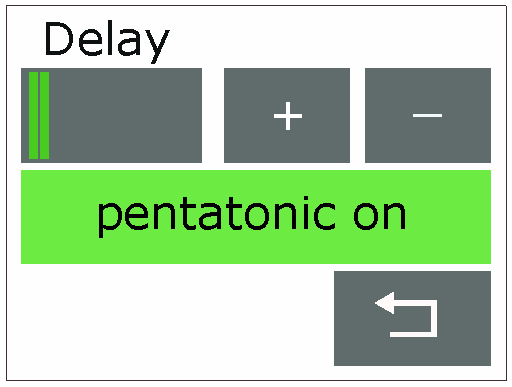
\includegraphics[width=0.3\textwidth]{settings.pdf}
	}
	\\
	\subfloat[Play help Menu\label{img:play_help_screen}]{%
		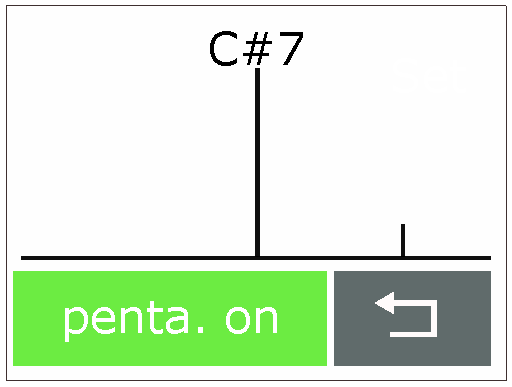
\includegraphics[width=0.3\textwidth]{pitch_display.pdf}
	}
	\hfill

	\caption{Dummy figure}
	\label{fig:dummy}
\end{figure}

	\subsection{Treiber}\label{subsec:drivers}
In diesem Unterkapitel sind die verschiedenen Funktionen der selbst geschriebenen Treiber für die Custom IP Komponenten Tonhöhenverarbeitung und Lautstärkeverarbeitung beschrieben. Zusätzlich war die Erstellung eines Treiber für den LT24 Controller nötig, da Terasic den zur Verfügung gestellten Treiber nicht nach den Konventionen von Intel erstellt hat.

Um ein selbst erstellten Treiber dem Board Support Package (BSP) hinzuzufügen, müssen die Benennungen und Ablageorte der Files einige Bedingungen erfüllen.  
Die Treiber Dateien müssen in dem Ordner IP abgelegt sein, welcher sich im Quartus Projekt Ordner befinden muss. Darin muss ein Skript mit der Endung sw.tcl abgelegt sein. In diesem Skript muss ein eindeutiger Name für den Treiber angegeben sein. Zudem muss der Pfad zu den Treiber Daten angegeben sein. Intel empfiehlt drei Treiber Daten zu erstellen:
  \renewcommand{\labelitemi}{$\blacksquare$}
 \renewcommand\labelitemii{$\square$}
 \begin{itemize}
 	\item  inc
 	\begin{itemize}
 		\item  custom\_ip\_regs.h
 	\end{itemize}
 \end{itemize}
 \begin{itemize}
	\item  HAL
	\begin{itemize}
		\item  custom\_ip\_.h
		\item  custom\_ip\_.c
	\end{itemize}
\end{itemize}

Das File mit der Endung regs.h definiert Hardware Interface spezifische Abläufe. Dieses wird im Ordner inc abgelegt. Im HAL Ordner sind ein c und ein h File erstellt, welche die Integration mit dem Hardware Abstracten Layer(HAL) ermöglichen \cite{NIOS_II_soft}.
Die folgenden Paragraphe zeigen die in den c Dateien realisierten Funktionen für die drei Treiber.

\paragraph{LT24 Controller}\mbox{}\\

Wie in der Einleitung dieses Unterkapitels erwähnt erfüllt der von Terasic mitgelieferte Treiber nicht die Konventionen welche Intel verlangt. Zudem sind die meisten Funktionen des Treibers sehr ineffizient gestaltet. Darum haben wir uns entschieden den Treiber für den LT24 Controller selbst zu schreiben. Im folgenden Teil ist beschrieben welche Funktionen es für die Steuerung des LCD gibt.

Das Modul \textit{LT24\_Controller.c} ermöglicht es auf dem LCD einzelne Pixel und Rechteckflächen zu zeichnen und zu löschen. Die Funktion \textit{LCD\_DrawPoint(x,y,color)} setzt ein Cursor an die gewünschte Stelle auf dem LCD und zeichnet ein Pixel in der entsprechenden Farbe. Auf diese Art ein Rechteck zu zeichnen ist sehr ineffizient. Da der Treiber von Terasic Rechtecke auf diese Art zeichnet, war eine effizientere Lösung nötig. Mit der Funktion \textit{LCD\_DrawRect(xs,ys,xe,ye,color)} werden Rechtecke effizienter gezeichnet. Es wird dabei nur einmal für das ganze Rechteck ein Cursor Feld aufgespannt und danach alle Pixel eingefärbt. Da durch das Cursor Feld nicht für jedes einzelne Pixel ein Cursor gesetzt werden muss, wird Zeit eingespart. 

\paragraph{Tonhöhenverarbeitung}\mbox{}\\

Das Modul \textit{Pitch\_generation.c} ermöglicht auf die Register aus Kapitel \ref{subsec:Pitch_Generation} zuzugreifen.
Die Funktion \textit{get\_pixel\_pitch\_accuracy(penta\_on\_off,pitch\_freq)} liesst das freq\_data Register aus. Dessen Wert wird für die Anzeige der Spielgenauigkeit in Abbildung \ref{img:play_help_screen} benötigt. Die Funktion berechnet aus dem gemessenen Frequenzwert und dem anzunähernden Ton einen Pixelwert um den senkrechten Strich auf dem Display einzuzeichnen.


\paragraph{Lautstärkenverarbeitung}\mbox{}\\
Die einzige Kommunikation welche die Lautstärkeverarbeitung Komponente mit dem NIOS II hat, ist das schreiben und lesen des Kontroll Registers um die Kalibrierung zu starten und um die Bedienung über die Antenne zu aktivieren oder deaktivieren. Das Modul \textit{Volume\_generation.c} ermöglicht dies. 
	\subsection{Audio}\label{subsec:audio}

Die Kommunikation mit WM8731 Codec geschieht über die IP Componente Audi\_Video Configuration von Intel. Diese besitzt die Funktion 
\textit{alt\_up\_av\_config\_write\_audio\_cfg\_register} um die Kontrollregister des Codec über den Hardware Abstraction Layer (HAL) anzusprechen\cite{Audio_config}.
Das Module \textbf{audio.c} beinhaltet die beiden Funktionen, \textit{codec\_wm8731\_init()} und \textit{set\_vol(vol\_gain)}. 

In der Initialisierung wird der Codec als Master konfiguriert. Der Clock des Codec wird auf \SI{12}{MHz} gesetzt und die Sampling Rate auf \SI{48}{kHz}. Die Input Audio Data Bit Länge wird auf 24 Bit gesetzt und der Übertragungsmodus der Daten auf left justified gesetzt. Mit diesen Einstellungen ist eine Kominikation mit der audio serializer Komponente möglich \todo{Verweiss auf Dennis}.
Um Störungen zu vermeiden sind die Line In Eingänge des Codec gemutet, da wir nur den Line Out brauchen. Der Linke und Rechte Kanal sind so eingestellt das beide Kanäle die selben Lautstärken haben\cite{codec}. 

Die Gesamtlautstärke des Theremin ist auf 10 unterschiedliche Pegel einbestellbar, dies geschieht mit dem Aufruf der Funktion \textit{set\_vol(vol\_gain)}. Die leiseste Stufe dämpft den Audio Signal Pegel um \SI{-76}{db}. Jeweils eine Stufe grösser reduziert die Dämpfung um \SI{7}{db}. Die höchste Stufe dämpft den Audio Signal Pegel um \SI{-7}{db}. Der Codec könnte gemäss Datenblatt das Signal bis +6dB verstärken. Nach Labor Tests haben wir uns entschieden das Audio Signal nur zu dämpfen, da eine Verstärkung zu laut ist.


Ursprünglich war geplant die Lautstärke Einstellung der Volume Antenne über den Codec zu steuern. Nicht wie in Kapitel \ref{subsec:Volume_Generation} beschrieben über die VHDL Komponente. Diese Methode konnte jedoch nicht realisier werden, da die Zero Cross detection des Codec nicht funktionierte. Mit der Zero Cross Dedection sollte der Codec erst bei einem Nulldurchgang die Lautstärke vermindern oder erhöhen. In unseren Versuchen hat sich die Lautstärke jedoch nie geändert, obwohl ein Sinus Audio Signal angelegt wurde. Wir mussten feststellen das diese Methode für den DAC nicht funktioniert. Mit dieser Methode hätte die Lautstärke, verglichen zur realisierten Methode, eine bessere Dynamik gehabt. \today{genauer erklären}
	\subsection{Touch}\label{subsec:touch}
 Die von Terasic zur Verfügung gestellte Datei zur auslesen des Touch ist leider sehr unübersichtlich aufgebaut. Es ist sehr schwierig die darin enthaltenen Funktionen auf unser Projekt anzuwenden. Daher entschieden wir uns selbst ein Touch Interrupt Routine zu erstellen. 
 
 Der resistive Touch Display des LT24 LCD touch module ist mit dem AD783 Analoge Devices Chip verbunden. Sobald der Touch Display berührt wird lösst der Chip am Pen Interrupt Pin ein Interrupt aus welches vom NIOS II detektiert wird. Der AD783 Chip speicher die X und Y Koordinaten zum Zeitpunkt des Interrupts ab. Diese können über den SPI Bus ausgelesen werden\cite{AD7843}. 
 
 Für unser Projekt sind wir daran interessiert den Pen Interrupt zu detektieren und die X und Y Koordinaten auszulesen, damit wir sagen können welcher Taster gedrückt worden ist.
 
Das ganze ist im Modul \textit{touch\_isr.c} realisiert. Darin befindet sich eine Funktion \\ \textit{touch\_init(void*context)}. Diese aktiviert das Touch Pen Interrupt  und registriert die Funktion welche durch das Interrupt aufgerufen wird. 
In der Interrupt Funktion \textit{touch\_isr(void*context)} wird zuerst das Touch Pen Interrupt  deaktiviert. So das in dieser Zeit kein weiteres Interrupt auftreten kann. Nach dem deaktivieren des Interrupts liesst der \textit{alt\_avalon\_spi\_command} die X und Y Koordinaten aus.
	\subsection{GUI}\label{subsec:gui}
Die Funktionen, welche von Terasic für die Gestaltung des GUI zur Verfügung gestellt werden, sind für unser Projekt zu ineffizient. Um einen Text anzuzeigen, verwendet Terasic eine Funktion, die ein Alpha Blending an den Rändern der Buchstaben durchführt. Dabei wird die Schriftfarbe mit der Hintergrundfarbe gemischt. Dieser Prozess nimmt viel Zeit in Anspruch und hat wenig Nutzen. Wodurch bei jedem neuen Zeichnen eines Texts zugeschaut werden konnte, wie die Pixel gezeichnet wurden. Dies ist für unser Projekt unbrauchbar. Zudem war eine ansprechendere Schriftart nötig. Daher realisierten wir eine eigene Funktion, welche Texte zeichnet. Diese ist im Modul \textbf{simple\_text.c} umgesetzt.

\paragraph{simple\_text.c}\mbox{}\\

Mit dem Open Source Tool ''The Dot Factory`` liess sich eine Bitmap für die Schrifftart Arial generieren, welche 22 Punkte gross gewählt ist. Das Tool generiert zwei Arrays. Im Bitmap Array sind die Buchstaben in einer Bitmap gespeichert. Das Descriptor Array enthält Informationen über die Breite jedes Characters und den Offset in der Character Bitmap. Um den Offset eines Buchstabens zu bestimmen, wird der Character minus des ersten Characters in der Bitmap gerechnet. Dies ergibt den Index für das Descriptor Array, in welchem der Offset für die Bitmap gespeichert ist. In Abbildung \ref{img:bitmap} ist dieser Prozess veranschaulicht. In diesem Beispiel besteht die Bitmap aus den Buchstaben a, b und c. Für den Buchstaben b wird der Offset 1 ausgerechnet. Im Descriptor Arrey ist auf Position 1 die Breite 5 gespeichert und der Offset 10 für die Bitmap. Mit diesen Informationen kann die Funktion \textit{print\_string(x,y,color,font,font\_descriptor,string)} einen Text String zeichnen. Dabei werden nur die Pixel gezeichnet, welche in der Bitmap auf 1 gesetzt sind.

\begin{figure}[h]
	\centering
	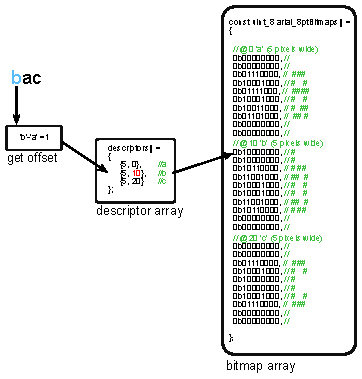
\includegraphics[width=0.8\textwidth]{the_dot_factory.pdf}
	\caption{Bitmap und Discriptor Array.}
	\label{img:bitmap}
\end{figure}

\paragraph{gui.c} \mbox{}\\

In diesem Modul sind mit der Funktion \textit{print\_string(x,y,color,font,font\_descriptor,string)} aus dem Modul  \textit{simple\_text.c} und der Funktion \textit{LCD\_DrawRect(xs,ys,xe,ye,color)} aus dem Modul \textit{LT24\_controller.c} die einzelnen Menüs dargestellt. 
	\subsection{Lizenzen}\label{subsec:Lizenzen}
Der Hardware Abstraction Layer (HAL) verwendet die Open-Source C standart Bibliothek \textit{newlib}. Es ist nicht erforderlich den Quellcode zu veröffentlichen\cite{NIOS_II_soft}.

Das verwendete Tool um die Bitmaps der Buchstaben zu erzeugen, "The Dot Factory", ist MIT lizenziert. Es ist ebenfalls nicht erforderlich den Quellcode zu veröffentlichen. 

\pagebreak

\clearpage
\section{Realisierung Gehäuse}\label{sec:Realisierung Gehäuse}
Im folgenden Teil des Fachberichtes ist die Realisierung des Gehäuses beschrieben. 

Die Anforderungen an das Gehäuse des digitalen Theremins sind:
\begin{itemize}
	\item Die Lautstärken- und die Tonhöhenantenne müssen genügend Abstand zueinander haben, damit der Spieler das Theremin richtig spielen kann.
	\item Das Antennenoszillator PCB und das DE1-SoC Board müssen für den Spieler ersichtlich sein.
	\item Für die Bedienung muss das LT24 Touch Modul für den Benutzer gut sichtbar platziert sein.
	\item Um den Preis des Gehäuses tief zu halten und für die Gestaltung des Gehäuses möglichst viel Freiheit zu haben, soll das Gehäuse 3D-gedruckt sein.  
\end{itemize}

Um diese Anforderungen zu erfüllen, konstruierten wir das Gehäuse mit dem 3D-CAD-System Inventor. Inventor ist eine sehr umfangreiche Konstruktions-Software mit dem die ausgefallene Form des Gehäuses leicht zu realisieren war.
Um das Gehäuse zu drucken, verwendeten wir den S5 Ultimaker 3D Drucker, da dieser sehr benutzerfreundlich ist und ein grosses Druckvolumen hat. 
Der S5 Drucker hat eine Druckvolumen von \SI{330x240x300}{mm}. 
Das Gehäuse musste jedoch in vier Teile unterteilt werden, damit die Platzverhältnisse im Drucker ausreichten. 

Wir gestalteten die Form des Theremins oval, da andere kommerziell erhältliche Theremins eine solche Form aufweisen. Die vier Einzelteile des Gehäuses sind alle gleich aufgebaut. Abbildung \ref{img:grundteil} zeigt die Grundstruktur eines Einzelteils. Die Funktion Wandung von Inventor ermöglichte es, die Grundstruktur oval auszuhöhlen. Jeweils zwei Einzelteile bilden zusammen den Deckel und den Boden. Daraus resultierte das in Abbildung \ref{img:Theremin_case} gezeigte Gehäuse. 

Die vier Einzelteile bestehen aus schwarzem Polylactide (PLA). Da das Gehäuse eine ovale Geometrie hat, braucht es Stützstrukturen für den Herstellungsprozess. Das eingesetzte Polyvinylalkohol (PVAL) hat die nützliche Eigenschaft, das es wasserlösslich ist.
\begin{figure}[h]
	\centering
	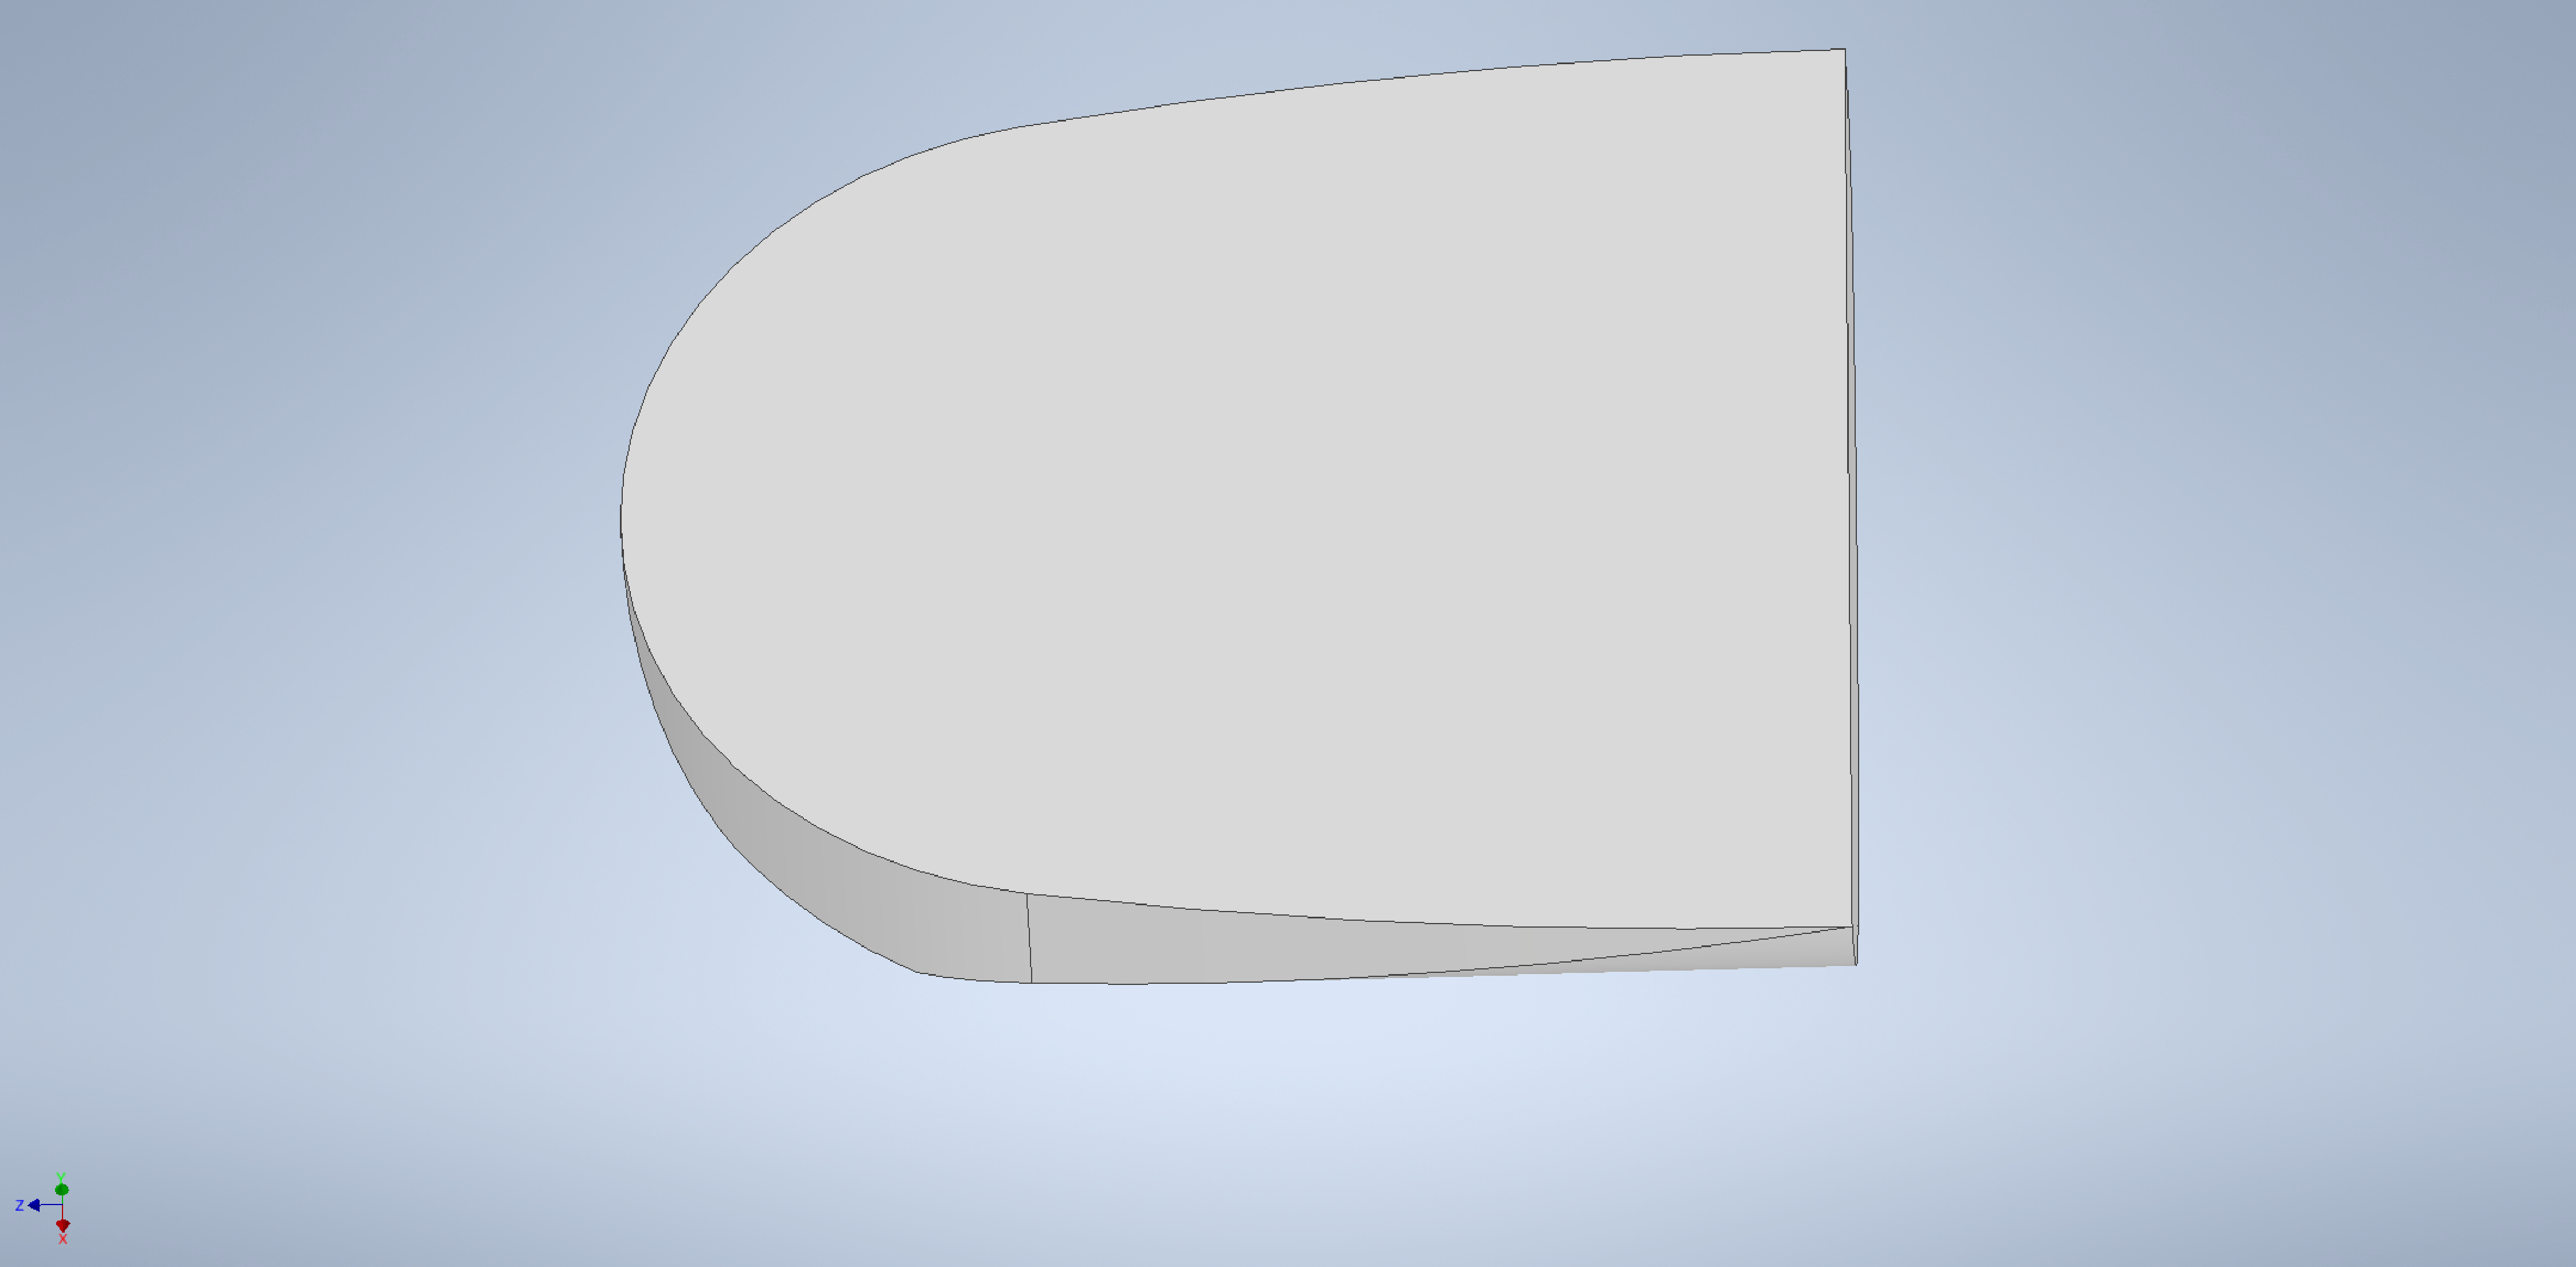
\includegraphics[width=\textwidth]{grundteil.pdf}
	\caption{Grundstruktur eines Einzelteils.}
	\label{img:grundteil}
\end{figure}
\begin{figure}[h]
	\centering
	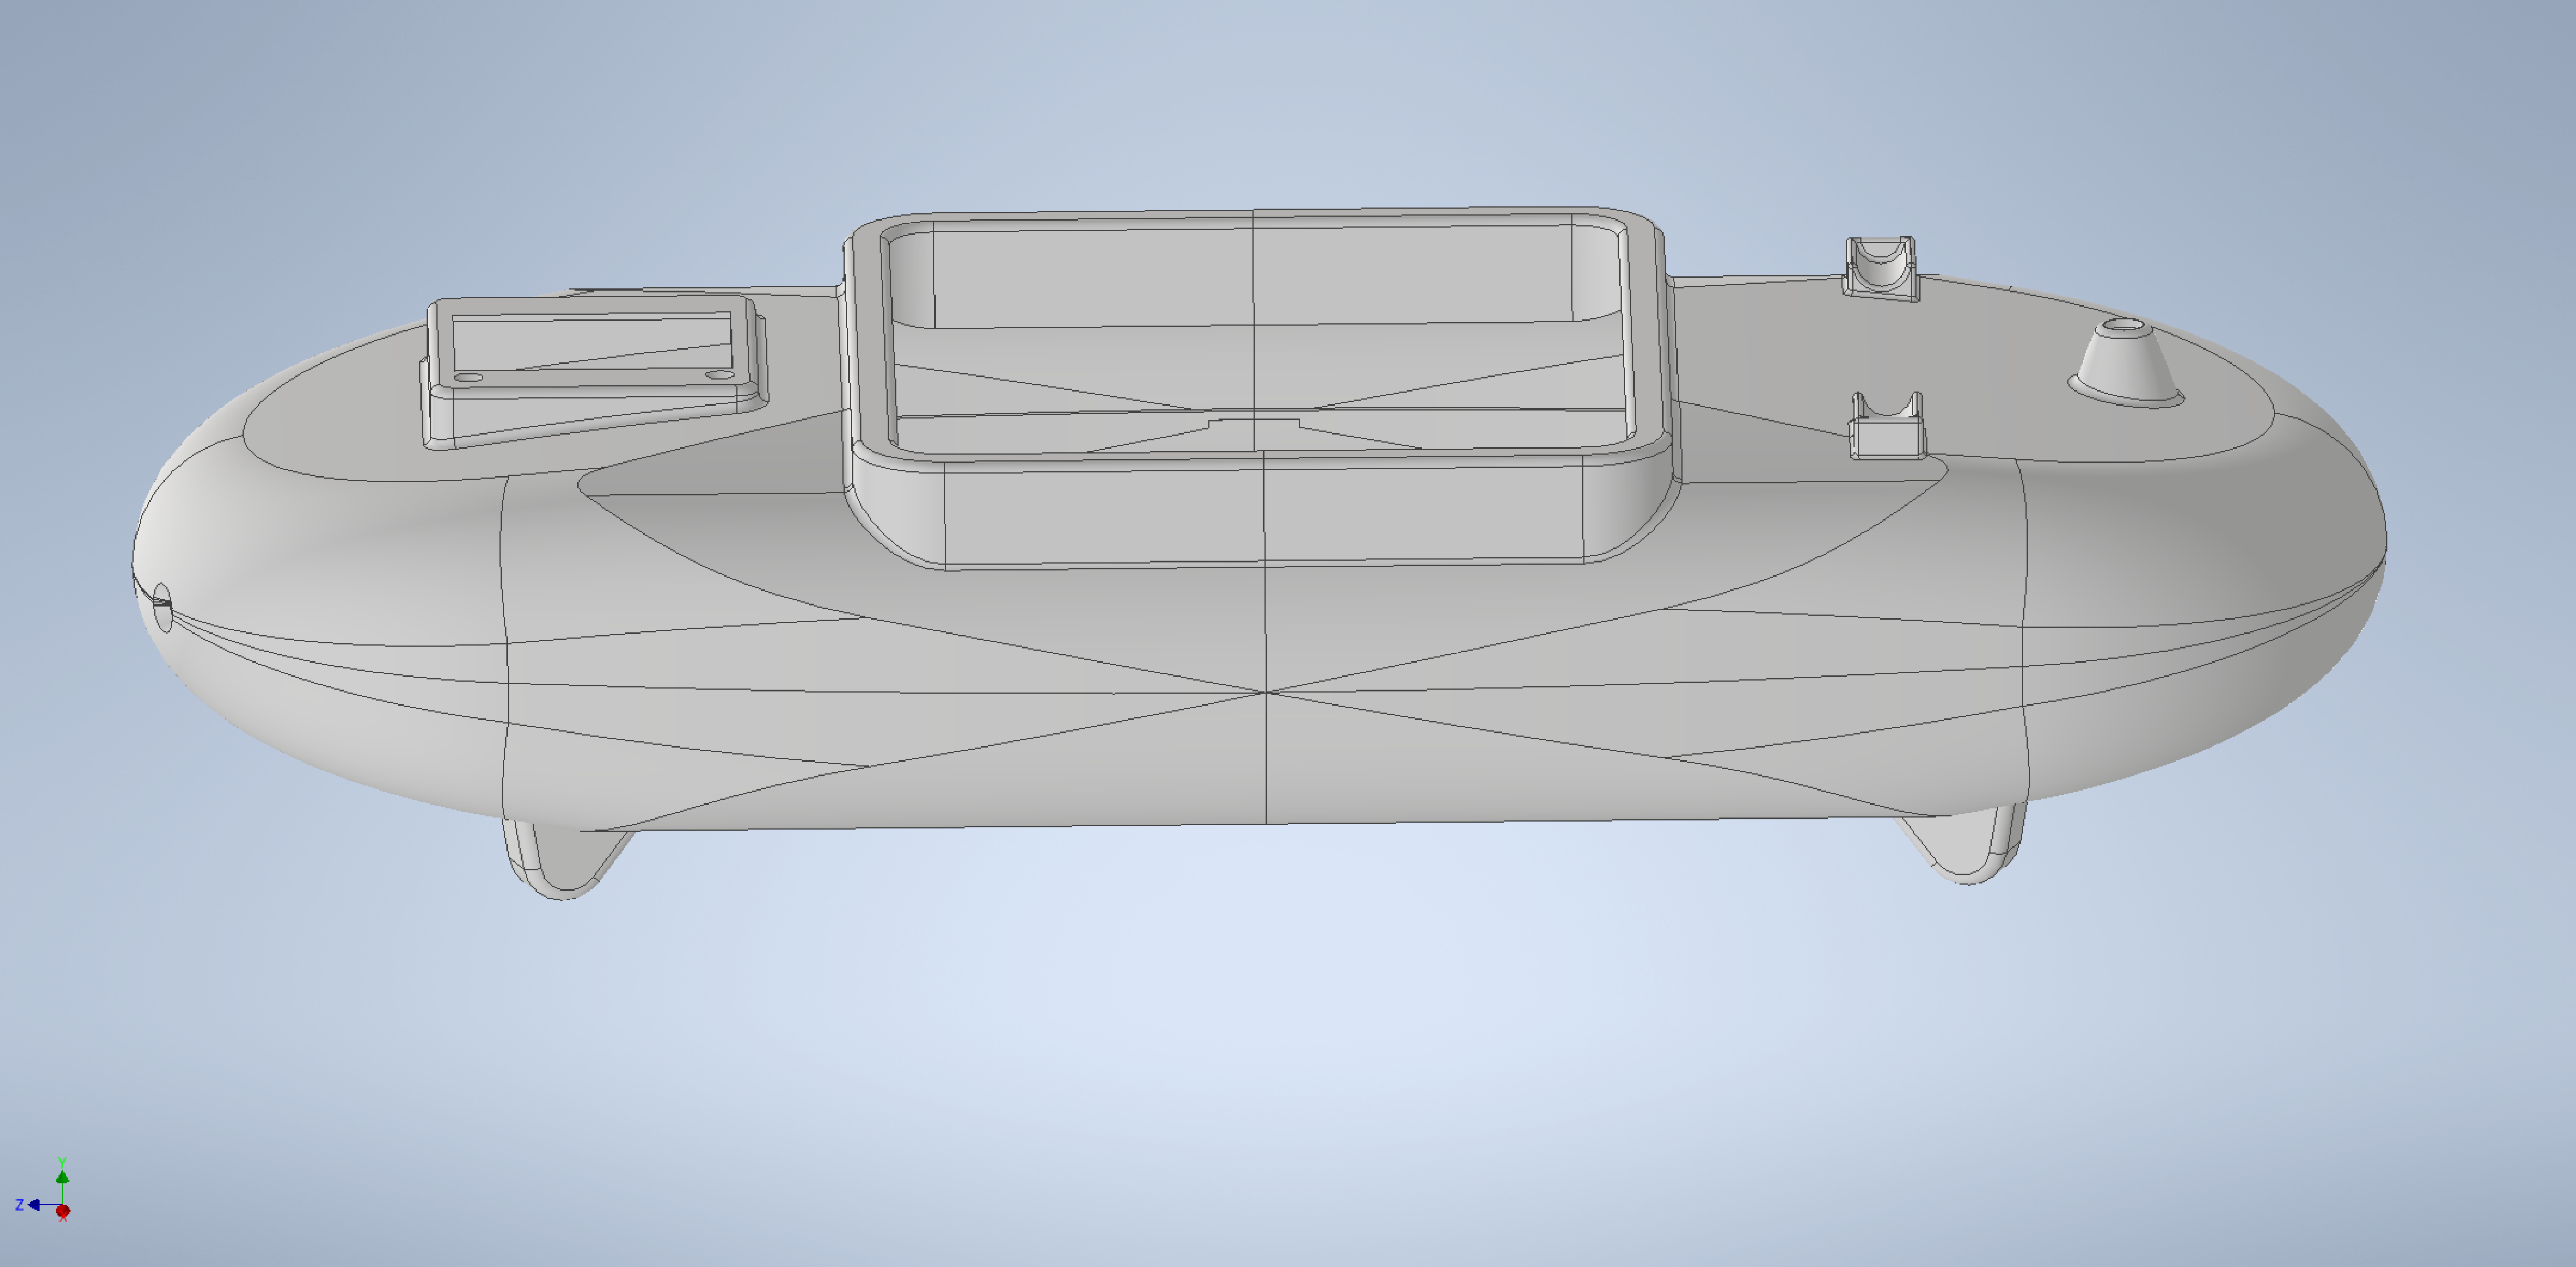
\includegraphics[width=\textwidth]{Theremin_case.pdf}
	\caption{Theremin-Gehäuse.}
	\label{img:Theremin_case}
\end{figure}





\pagebreak

\clearpage
\section{Validierung}\label{sec:Validierung}
In diesem Kapitel sind die Resultate der Messungen des PCB, der Frequenzmessung, des Glissando Effekts und des Ton Display aufgeführt. Dabei wird jeweils der Messaufbau beschrieben und die Resultate dargestellt und kommentiert. 
	\subsection{Antennenoszillator PCB}\label{subsec:PCB}
Auf dem Antennenoszillator PCB haben wir die Betriebsspannungen und die Ausgänge der Komperatoren getestet. Die dazu verwendeten Messmittel sind in Tabelle \ref{tab:Gemessene_Spannungen_PCB} angegeben. Die Signale haben wir mit dem Lecroy Wavesurfer 3054 Oszilloskop gemessen. 

Die \SI{9}{V} Betriebsspannung hat eine Rippelspannung von \SI{7.3}{mV}. Somit ist die Colpitts Oszillator-Schaltung stabil gespiesen. Die \SI{3.3}{V} Betriebsspannung weist eine Rippelspannung von \SI{133}{mV} auf. Dies ist jedoch noch vertretbar, da die Spannung für den digitalen Teil der Schaltung gebraucht wird.
\begin{table}[H]
	\centering
	\caption{Gemessene Spannungen PCB}
	\label{tab:Gemessene_Spannungen_PCB}
	\begin{tabular}{l|l|l|l}
		\textbf{Spannung} & \textbf{soll [VDC]} & \textbf{ist [VDC]} &	\textbf{Ripple [mVDC]}\\
		\hline \hline
		
		Betriebsspannung 9V & 9 & 9.3 &  7.3 \\ 
		&      &   &   \\ 
		\hline
		Betriebsspannung 3.3V & 3.3 & 3.4 &  133 \\ 
		&     &     &   \\ 
		\hline
		Schaltnetzteil 12V & 12 & 12.5 &  150 \\ 
		&     &       &   \\ 
		\hline
		
	\end{tabular}
\end{table} 

Bei den Messungen der Ausgänge der Komparatoren waren auf den Rechtecken bei der steigenden und fallenden Flanke Überschwinger ersichtlich. In einem Paper von Analog Device haben wir erfahren, dass die Verursacher der Überschwinger die langen Ausgangsleitungen sind. Diese wirken wie nicht abgeschlossene Übertragungsleitungen und lösen Reflexionen aus \cite{comparator_techniques}. Um dieses Problem zu lösen, schlossen wir die Ausgangsleitung mit einem \SI{300}{Ohm} Widerstand ab.

Beim ersten Austesten der Oszillatoren mit angeschlossenen Antennen wiesen die Oszillatoren ähnliche Frequenzen auf. Bei einer Veränderung der Lautstärkenoszillatorfrequenz wurde ebenfalls die Tonhöhenantennenfrequenz verändert. Dies kann durch Übersprechen oder gegenseitige Beeinflussung der Oszillatoren hervorgerufen werden. Um dieses Problem zu umgehen, haben wir die Frequenzen der beiden Oszillatoren um \SI{30}{kHz} versetzt zu gewählt. Dadurch war das Problem behoben. 

Durch den häufigen Gebrauch des PCB ist uns bewusst geworden, dass der verwendete JFet sehr empfindlich gegenüber elektrostatischer Entladung ist.

Bei einer Weiterentwicklung des Theremins sollte das Antennenoszillator PCB überarbeitet werden. Es ist eine Schutzbeschaltung für den JFet notwendig. Zudem sollten die Oszillatoren auf zwei separaten PCB realisiert werden, um Übersprechen und gegenseitige Beeinflussung zu vermeiden. 

\begin{table}[H]
	\centering
	\caption{Verwendete Messmittel}
	\label{tab:Verwendete_Messmittel}
	\begin{tabular}{l|l}
		\textbf{Messgerät} & \textbf{Bezeichnung}	\\
		\hline \hline
		
		Lecroy wavesurfer 3054  &  MSZ-M-0091  \\ 
		&        \\ 
		\hline
		
	\end{tabular}
\end{table} 
	\subsection{Frequenzmessung}\label{subsec:Frequenzmessung}
Um die Genauigkeit der Frequenzmessung zu bestimmen, testeten wir das Theremin bei den  Frequenzen aus der Tabelle \ref{tab:Toene_Frequenzen} in Kapitel \ref{subsec:Musiktheorie}.
 Wir verwendeten dazu anstatt unseres PCB einen Funktionsgenerator, da keine genaue Messung mit dem PCB möglich ist. Zum Auslesen der Frequenz nutzen wir das Tool \textit{SignalTap Logic Analyzer} in Quartus, um auf das Register der Frequenzmessung mit den Messresultaten zuzugreifen.
 Zu Beginn der Messung war eine Bestimmung des Offset des Referenzoszillators nötig. Der Frequenzgenerator wurde um \SI{120}{Hz} tiefer eingestellt als der Referenzoszillator, da \SI{120}{Hz} die Frequenz ist, auf die kalibriert wird. Daraus ergab sich ein Offset von  \SI{6}{Hz}.
 Für die Bestimmung der minimal und maximal gemessenen Frequenzwerte lasen wir aus dem SignalTap 20 Werte aus. Aus dem Maximum und Minimum bestimmten wir die grösste Abweichung zum entsprechenden Ton. Aus diesen Abweichungen berechneten wir die Werte aus Abbildung \ref{img:plot_frequenzmessung} .

 Alle gemessenen Werte liegen unter einem Fehler von 8 Cent. Wie bereits im Kapitel \ref{subsec:Musiktheorie} beschrieben, ist es schwer zu sagen, wann ein Ton als ''nicht getroffen`` empfunden wird. Daher haben wir uns darauf geeinigt, dass Werte unter 8 Cent als ''getroffen`` empfunden werden. Somit erfüllen alle Frequenzen diese Genauigkeit.
 
 Wie in Abbildung \ref{img:plot_frequenzmessung} ersichtlich, steigt die Messung mit zunehmender Frequenz immer mehr an. Dies spricht mit der Simulation aus Matlab aus Abbildung \ref{img:plot_freq_sim} überein. Dabei wurde in Matlab dieselbe Messmethode simuliert in \SI{1}{Hz} Schritten von \SI{100}{Hz} bis \SI{2}{kHz}. Auch die tiefen Cent Werte um \SI{600}{Hz} stimmen mit der Simulation überein, da gewisse Frequenzen mit der gewählten Abtastfrequenz von \SI{1.2}{MHz} eine genauere Messung ergeben.
 \begin{figure}[h]
 	\centering
 	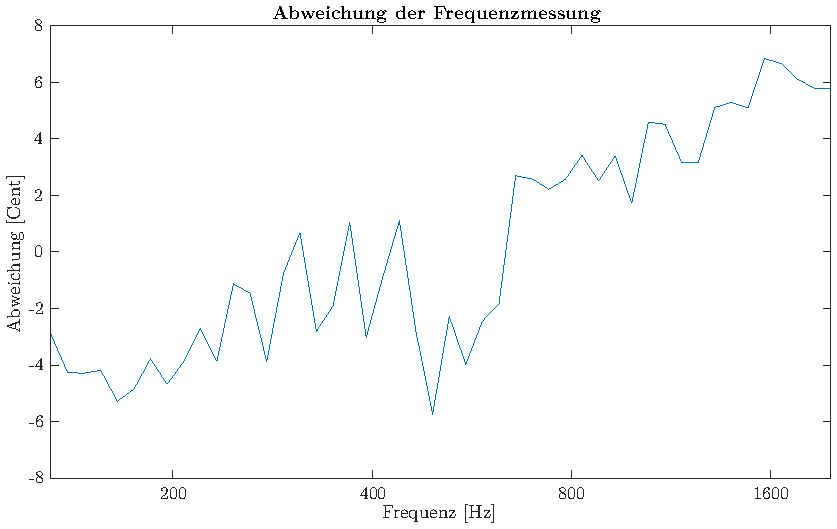
\includegraphics[width=0.9\textwidth]{Validierung_frequenzmessung.pdf}
 	\caption{Maximale Abweichung der Frequenzmessung.}
 	\label{img:plot_frequenzmessung}
 \end{figure}
 \begin{figure}[h]
	\centering
	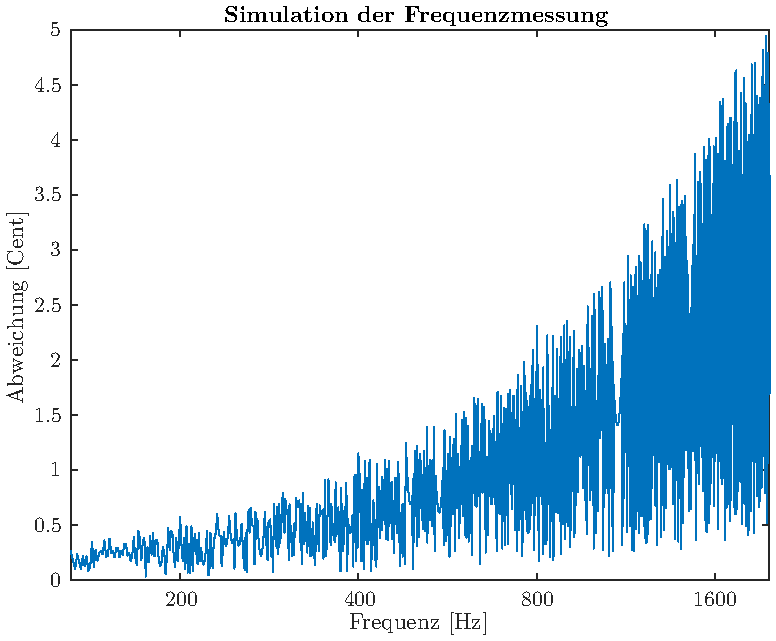
\includegraphics[width=0.9\textwidth]{Simulation_Frequenzmessung.pdf}
	\caption{Abweichung der Frequenzmessung in der Simulation}
	\label{img:plot_freq_sim}
\end{figure}
\begin{table}[H]
	\centering
	\caption{Verwendete Messmittel}
	\label{tab:Verwendete_Messmittel_freq}
	\begin{tabular}{l|l}
		\textbf{Messgerät} & \textbf{Bezeichnung}	\\
		\hline \hline
		
		Funktionsgenerator  & MSZ-M-0051   \\ 
		&        \\ 
		\hline
		SignalTap Logic Analyzer  &    \\ 
		&        \\ 
			\hline
	\end{tabular}
\end{table} 

\pagebreak

	\subsection{Glissando Effekt}\label{subsec:Glissando_Effekt}
Auch für den Glissando-Effekt war es nötig einen Test durchzuführen um die Genauigkeit der Töne festzustellen. Wir verwendeten auch hier anstatt unseres PCB einen Funktionsgenerator. Um die Frequenz einzustellen, wurde das Tool \textit{SignalTap Logic Analyzer} in Quartus eingesetzt um auf das Register der Frequenzmessung mit den Messresultaten zuzugreifen. Schlussendlich wurde der Ton mit der App \textit{Tonal Energy Tuner} auf dessen Genauigkeit gemessen. Die App gibt diese Genauigkeit direkt in Cent an. Die Messung umfasst alle Frequenzen aus der Tabelle \ref{tab:Toene_Frequenzen} in Kapitel \ref{subsec:Musiktheorie}. In Abbildung \ref{img:Validierung_Glissando} sind alle diese Abweichungen aufgezeigt. Die blaue Kurve  zeigt die Resultate, wenn die Frequenz kleiner eingestellt wurde als der anzunähernde Ton. Die orange Kurve zeigt die Resultate, wenn die Frequenz grösser eingestellt wurde als der anzunähernde Ton. Wie zu sehen ist, ist auch diese Funktion genauer als \SI{8}{Cent}. Interessanterweise nimmt bei beiden Einstellungen offenbar die angenäherte Frequenz mit höheren Tönen immer mehr ab. Da die Frequenzmessung wie zuvor besprochen mit grösseren Frequenzen immer mehr Abweichung hat ist dies auch erklärbar.\\
Weshalb die Kurve nicht wie in der Frequenzmessung immer mehr positiv wird erklärt die Abbildung \ref{img:Erklaerung_Glissando}. Da bei tiefen Frequenzen die gemessene Frequenz eher tiefer ist als die wirkliche bedeutet dies, dass der ist-Wert grösser ist als der Messungs-Wert. Der Glissando-Effekt nähert nun die Differenz zwischen dem gemessenen Wert und dem soll-Wert an. Dies bedeutet dass der angenäherte Wert jedoch immer noch die Abweichung zwischen ist und Messung hat. Bei den hohen Frequenzen ist es genau umgekehrt. Die Messung ist nun höher im Vergleich zum ist-Wert. Somit bewirkt der Glissando-Effekt in diesem Szenario, dass die angenäherte Frequenz kleiner ist als der soll-Wert.


\begin{figure}[h!]
	\centering
	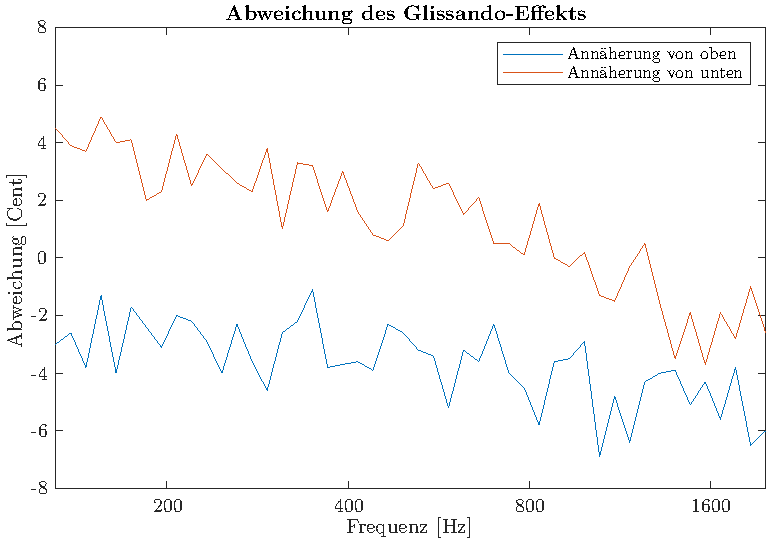
\includegraphics[width=0.9\textwidth]{Validierung_Glissando.pdf}
	\caption{Resultate der Validierung des Glissando-Effekts} 
	\label{img:Validierung_Glissando}
\end{figure}  

\begin{figure}[h!]
	\centering
	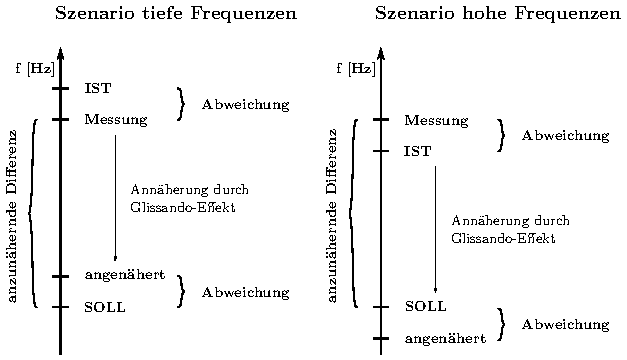
\includegraphics[width=0.9\textwidth]{Erklaerung_Glissando.pdf}
	\caption{Erklärung der beobachteten Änderungen} 
	\label{img:Erklaerung_Glissando}
\end{figure} 

\begin{table}[H]
	\centering
	\caption{verwendete Messmittel}
	\label{tab:Glissando_Messmittel}
	\begin{tabular}{l|l|l}
		\textbf{Messmittel} & \textbf{Bezeichnung} \\
		\hline\hline
		Funktionsgenerator & MSZ-M-0051   \\ \hline
		SignalTap Logic Analyzer & -    \\ \hline
		Tonal Energy Tuner App &  -   \\ \hline
		
	\end{tabular}
\end{table}


	\subsection{Gesamttest}\label{subsec:Gesammttest}
Zuletzt haben wir den gesamten Aufbau auf dessen Funktionsfähigkeit getestet. Dabei sind drei Punkte aufgefallen.\\
Erstens tritt das leichte Aliasing, welches zu erwarten war, bei hoher Lautstärke auf. Auffallend ist, dass dieses nur bei den höheren Tönen (über \SI{1}{kHz}) auftritt. Dies ist auf die Filterung des Mischersignals durch die CIC-Filter und das verwenden eines Rechtecksignals im Mischer zurückzuführen. Die Oberwellen des Rechtecksignals, welche auch Mischprodukte hervorrufen, machen es schwierig, durch Filterung mittels CIC-Filter Aliasing ganz zu vermeiden. Diese Problematik ist in Kapitel \ref{subsec:CIC_Filter} beschrieben.\\
Zweitens ist bei einer bestimmten Einstellung des Theremins ein Rauschen zu hören. Stellt man die Lautstärke auf dem Display auf das Maximum und über die Lautstärkenantenne eine tiefe Lautstärke ein, ist ein leichtes Rauschen zu hören. Dies ist auf den Kompromiss, auf welchen wir in Kapitel \ref{subsec:audio} eingegangen sind, zurückzuführen. Da der Digital-Analog-Wandler im Codec in diesem Fall ein nicht voll ausgesteuertes digitales Signal erhält, fällt dessen Rauschen mehr ins Gewicht.\\
Weiter ist erst nach der nicht flüchtigen Programmierung des Theremins aufgefallen, dass wenn das USB Kabel ausgesteckt wird, das Theremin nicht mehr funktioniert. Dies liegt darin, dass das verwendete Netzteil keinen Erdungsanschluss hat. Während den Tests war das Entwicklungsboard ständig über das USB-Kabel und den angeschlossenen PC geerdet. Nachdem das Theremin separat über einen Stecker eine Erdung erhielt, war dieses Problem verschwunden.



\pagebreak

\clearpage
\section{Erfahrungen}\label{sec:Erfahrungen}

Über das 5 und 6 Semester haben wir einige Erfahrungen mit Intel FPGA  sammeln können. In diesem Abschnitt berichten wir über unsere Erfahrungen und Eindrücke der verwendeten Tools.





\pagebreak
\clearpage
\section{Schlusswort}\label{sec:Schlusswort}
Das Projekt 6 umfasste die abschliessende Entwicklung eines digitalen Theremins auf einem FPGA. Die Grundlagen für die Weiterentwicklung stammen aus der Arbeit des Projektes 5 ein Semester zuvor. Diese Grundlagen beinhalteten die Verarbeitung des Antennensignals. 

\paragraph{Ergebnisse}\mbox{}\\

Die Implementierung der Lautstärkensteuerung über eine zweite Antenne ist abgeschlossen und funktioniert einwandfrei. 
Damit diese auch ein Signal erhält, ist der zweite analoge Oszillator in einem Redesign des PCB hinzugefügt worden. Dieses Redesign umfasst nebst des zweiten Oszillators eine Speisung der beiden Schaltungen über das gleiche Netzteil wie das FPGA.

Die Bedienung des FPGA läuft über den implementierten Nios II Prozessor und den von ihm gesteuerten LCD Display. Der Benutzer kann über den Touchscreen diverse Einstellungen vornehmen und Funktionen des Theremins einfach aktivieren und deaktivieren.

Der Spieler kann die automatische Kalibration des Theremins über das Menu starten, um es auf seinen Spielstil abzustimmen. Dazu gleicht das Theremin die beiden digitalen Referenzoszillatoren auf die analogen Antennenoszillatoren ab.

Das Spielen von genauen Tönen ist nun auch möglich, wenn der Spieler keine ruhige Hand hat. Der eingebaute Glissando-Effekt korrigiert während dem Spielen die Töne auf den nächstgelegenen Ton. Gespielt werden kann in zwei Tonsystemen: normale Tonleiter mit Halbtönen oder eine pentatonische Tonleiter. Die pentatonische Tonleiter ist praktisch, um ohne grossen Aufwand ansprechend klingende Melodien zu spielen. 

Während dem Spielen ermöglicht es die Anzeige der Spielgenauigkeit zu sehen, wie falsch der Spieler seine Hand hält, wenn die pentatonische Tonleiter aktiv ist. Wenn die normale Tonleiter aktiviert ist, wird der nächstgelegene Ton angezeigt. Dies hilft denjenigen Spielern mit weniger musikalischen Talenten.

Schlussendlich wurde das Gerät in ein ansprechendes Gehäuse verpackt. Damit wir ein etwas ausgefalleneres Gehäuse fertigen konnten, entschieden wir uns dieses mit einem 3D-Drucker herzustellen.

\paragraph{Schwierigkeiten}\mbox{}\\

Weil wir viel Zeit für die Inbetriebnahme der ganzen Signalverarbeitung benötigten und wegen Umwelteinflüssen ausserhalb unserer Kontrolle, konnten wir die zusätzlichen Klangeffekte nicht implementieren.\\
Weiter ist beim Spielen bei höheren Frequenzen ein leichtes Aliasing zu hören, was auf den Aufbau der Filter zurückzuführen ist. Die Filter sind so eingestellt, dass dieses Aliasing möglichst minimiert ist.\\
Zuletzt kann bei der höchsten Lautstärkeneinstellung auf dem Display und der tiefsten Einstellung über die entsprechende Antenne ein Rauschen gehört werden. Dies ist auf die Implementierung der Lautstärkeneinstellung zurückzuführen. Bei dieser mussten wir wegen Schwierigkeiten mit dem verbauten Codec, Kompromisse eingehen.

\paragraph{Weiterentwicklung}\mbox{}\\

Das Aliasingproblem könnte durch die Verwendung eines Analog-Digital-Wandlers verkleinert werden. Dies da ein Analog-Digital-Wandler anstelle des Rechtecksignals direkt den Sinus des analogen Oszillators einlesen könnte. Die Multiplikation der Sinusse des Referenzoszillators und des analogen Oszillators würde nur eine hochfrequente Komponente bedeuten ohne Oberwellen. Nötig wäre dazu jedoch ein Wandler mit sehr hoher Abtastfrequenz.

Die Verwendung eines neuen Codec, mit welchem Nullstellenerkennung möglich wäre, ist ein Entfernen des Rauschens erreichbar, welches bei bestimmten Gegebenheiten hörbar ist.

Für die zwei zuvor genannten Verbesserungen ist ein Redesign des PCB nötig, bei dem eine Überarbeitung der Oszillatoren nötig ist. Eine Schutzbeschaltung der JFet ist nötig um diese vor statischer Entladung zu schützen.

\paragraph{Lerngewinn} \mbox{}\\

Bei der Projektwahl haben wir das digitale Theremin gewählt, um das erlernte Wissen über VHDL auszubauen und zu festigen. Über die letzten zwei Semester haben wir einige Erfahrungen im Umgang mit VHDL-Design und der Implementierung des NIOS II Softcores gesammelt.

Im Umgang mit Audio- und Signalverarbeitung haben wir gelernt darauf zu achten, das die Clocks dieser Komponenten vom gleichen Referenz Clock abgeleitet sein müssen. Dies hat zur Folge das die Komponenten synchron laufen. Dadurch kann es nicht vorkommen, dass eine Komponente das Signal schneller verarbeitet als die andere oder dass Daten verloren gehen. 

Im Umgang mit CIC Filtern haben wir gesehen, dass diese sehr praktisch sind. Jedoch müssen die Nullstellen in der Übertragungsfunktion berücksichtigt werden, da Signale in diesen Bereichen Aliasing verursachen. Der Einfluss der Nullstellen kann durch den Einsatz von mehreren CIC-Filtern mit kleinem Dezimationsfaktor verringert werden.


\pagebreak
\clearpage
\section{Danksagung}\label{sec:Danksagung}

In erster Linie möchten wir uns bei unserem Projektbetreuer Herrn Schenk und unserem Auftraggeber Herrn Hanspeter Schmid für Ihre Unterstützung während der vergangenen zwei Projekten bedanken. Mit ihrem Fachwissen und Ihren Ideen haben sie uns geholfen verschiedenste Problemstellungen zu meistern. 

Ebenfalls möchten wir uns bei den Mitarbeitern des ISE bedanken. Insbesondere Herrn Pichler und Herrn Zardet die uns in FPGA Design Fragen unterstützten.

Besonders möchten wir uns auch bei Herrn Stefan Muhr bedanken. Material und PCB Bestellungen wurden von ihm jeweils inert rekordverdächtig kurzer Zeit bearbeitet. Auch bei anderen Anliegen bezüglich Messgeräten und Bauteilen hat er uns stets aufgeholfen und mit seiner positiven Einstellung zu einem guten Arbeitsklima beigetragen.  

Zudem möchten wir uns bei Herrn Patrick Specht bedanken, für die nützlichen Tipps die er uns gegeben hat bezüglich 3D Druck.





\pagebreak
\section{Ehrlichkeitserklärung}\label{sec:Ehrlichkeitserklärung}
Mit der Unterschrift bestätigen die Unterzeichnenden Teammitglieder, dass die vorliegende Projektdokumentation selbstständig im Team und ohne Verwendung anderer, als der angegebenen Hilfsmittel verfasst wurde, sämtliche verwendeten Quellen erwähnt und die gängigen Zitierregeln eingehalten wurden. Eine Überprüfung der Arbeit auf Plagiate mithilfe elektronischer Hilfsmittel darf vorgenommen werden.


\vspace{20mm}


\begin{center}
		\renewcommand{\arraystretch}{1}
	\begin{tabular}{lp{5em}l} 
  
		
		Unterschrift:   && Ort, Datum: \\
		&&\\
		\hspace{5cm}   && \hspace{5cm} \\\cline{1-1}\cline{3-3}
		&&\\
		&&\\
		Unterschrift:   && Ort, Datum: \\
		&&\\
		\hspace{5cm}   && \hspace{5cm} \\\cline{1-1}\cline{3-3}
		&&\\
		&&\\

  
  \ \\
 \end{tabular}
 \end{center}





\pagebreak


\clearpage
%%---BIBLIOGRAPHY------------------------------------------------------------------------
{\sloppypar
\printbibliography[heading=bibintoc]
\label{sec:lit}
%\selectlanguage{ngerman}				%ngerman or english
%\printbibliography
}

%%---APPENDIX----------------------------------------------------------------------------
\begin{appendix} 


\end{appendix}


%%---NOTES for DEBUG---------------------------------------------------------------------
\ifdraft{%Do this only if mode=draft
%%requires \usepackage{todonotes})
\newpage
\listoftodos[\section{Todo-Notes}]
\clearpage
}
{%Do this only if mode=final
}

\end{document}
